\chapter{Exercise solutions}

\section{Algebraic expressions}

\subsection{Exercise 1-1} %p. 9-10
% \begin{exercises}{}{
\begin{enumerate}[noitemsep, label=\textbf{\arabic*}. ] 
\item %If $a$ is an integer, $b$ is an integer and $c$ is irrational, which of the following are rational numbers? 
  \begin{enumerate}[itemsep=5pt, label=\textbf{(\alph*)} ] 
    \item rational
    \item rational
    \item rational
    \item irrational
    \end{enumerate}
\item %%If $\dfrac{a}{1}$ is a rational number, which of the following are valid values for $a$?
    \begin{enumerate}[itemsep=5pt, label=\textbf{(\alph*)} ] 
    \item valid
    \item valid
    \item invalid
    \item valid
    \end{enumerate}

 \item %Write the following as fractions:
    \begin{enumerate}[itemsep=5pt, label=\textbf{(\alph*)} ] 
    \item
    \item %
    \item %
    \item %
    \end{enumerate}
\item% Write the following using the recurring decimal notation:
    \begin{enumerate}[itemsep=5pt, label=\textbf{(\alph*)} ] 
    \item %
    \item %
    \item %
    \item %
    \end{enumerate}
\item %%Write the following in decimal form, using the recurring decimal notation:
    \begin{enumerate}[itemsep=5pt, label=\textbf{(\alph*)} ] 
    \item %
    \item %
    \item %
    \item %
    \end{enumerate}
\item %%Write the following decimals in fractional form:
    \begin{enumerate}[itemsep=5pt, label=\textbf{(\alph*)} ] 
    \item %
    \item %
    \item %
    \end{enumerate}
\end{enumerate}

% \end{exercises}

\subsection{Exercise 1-2} %p. 9-12
% \begin{exercises}{}
% {
% Use your calculator to write the following in decimal form, round off to $3$ decimal places:
\begin{enumerate}[itemsep=5pt, label=\textbf{\arabic*}. ]
 \item %
\item %
\item %
\item
\item %
\item %
\end{enumerate}
}
\end{exercises}

\subsection{Exercise 1-3} %p. 9-15

% \begin{exercises}{}
%  {
% Determine between which two consecutive integers the following numbers lie, without using a calculator:
\begin{enumerate}[itemsep=5pt, label=\textbf{\arabic*}. ]
\item %
\item %
\item %
\item %

\end{enumerate}

% \end{exercises}
\subsection{Exercise 1-4} %p. 19
% \begin{exercises}{}
% {
% Find the products of the following:

\begin{multicols}{2}
\begin{enumerate}[label=\textbf{\arabic*}., itemsep=5pt]
\item %
\item %$(y+5)(y+2) $
\item %$(2-t)(1-2t)$
\item %$(x-4)(x+4)$
\item %$ (2p+9)(3p+1)$
\item %$(3k-2)(k+6)$
\item %$(s+6)^2$
\item %$-(7-x)(7+x)$
\item %$(3x-1)(3x+1)$
\item %$(7k+2)(3-2k)$
\item %$(1-4x)^2$
\item %$(-3-y)(5-y)$
\item %$(8-x)(8+x)$
\item %$(9+x)^2$
\item % $(-2{y}^{2}-4y+11)(5y-12)$ 
\item % $(7{y}^{2}-6y-8)(-2y+2)$% 
\item %$(10{y}^{5}+3)(-2{y}^{2}-11y+2)$ 
\item %$(-12y-3)(12{y}^{2}-11y+3)$% 
\item %$(-10)(2{y}^{2}+8y+3)$ 
\item %$(2{y}^{6}+3{y}^{5})(-5y-12)$% 
\item %$(-7y+11)(-12y+3)$% 
\item %$(7y+3)(7{y}^{2}+3y+10)$% m
\item %$(9)(8{y}^{2}-2y+3)$ 
\item %$(-6{y}^{4}+11{y}^{2}+3y)(10y+4)(4y-4)$ 
\end{enumerate}
\end{multicols}
% }
% \end{exercises}
\subsection{Exercise 1-5} %p. 21
% \begin{exercises}{}
% {
% Find the highest common factors of the
% following pairs of terms:\par

\begin{multicols}{2}
\begin{enumerate}[label=\textbf{\arabic*}., itemsep=5pt]
\item %$6y;~18x$
\item %$12mn;~8n$
\item %$3st;~4su$ 
\item %$18kl;~9kp$
\item %$abc;~ac$% 
\item %$2xy;~4xyz$
\item %$3uv;~6u$ 
\item %$9xy;~15xz$
\item %$24xyz;~16yz$
\item %$3m;~45n$
\end{enumerate}
\end{multicols}
% }
% \end{exercises}

\subsection{Exercise 1-6} %p. 23
% \begin{exercises}{}{
% Factorise:
\begin{multicols}{2}
\begin{enumerate}[itemsep=5pt, label=\textbf{\arabic*}. ] 
\item %$2l+2w$
\item %$12x+32y$
\item %$6{x}^{2}+2x+10{x}^{3}$
\item %$2x{y}^{2}+x{y}^{2}z+3xy$
\item %$-2a{b}^{2}-4{a}^{2}b$
\item %$7a+4$ 
\item %$20a-10$ 
\item %$18ab-3bc$
\item %$12kj+18kq$ 
\item %$16{k}^{2}-4$ 
\item %$3{a}^{2}+6a-18$
\item %$-12a+24a^3$ 
\item %$-2ab-8a$ 
\item %$24kj-16{k}^{2}j$
\item %$-{a}^{2}b-{b}^{2}a$ 
\item %$12{k}^{2}j+24{k}^{2}{j}^{2}$ 
\item %$72{b}^{2}q-18{b}^{3}{q}^{2}$
\item %$4(y-3)+k(3-y)$ 
\item %$a^2(a-1)-25(a-1)$ 
\item %$bm(b+4)-6m(b+4)$
\item %${a}^{2}(a+7)+9(a+7)$ 
\item %$3b(b-4)-7(4-b)$ 
\item %${a}^{2}{b}^{2}{c}^{2}-1$
\end{enumerate}
\end{multicols}
% }
% \end{exercises}

\subsection{Exercise 1-7} %p. 26-27
% \begin{exercises}{}
% {
\begin{enumerate}[itemsep=5pt, label=\textbf{\arabic*}. ] 
\item %%Factorise the following:
\begin{multicols}{2}
\begin{enumerate}[itemsep=5pt, label=\textbf{(\alph*)} ] 
\item %${x}^{2}+8x+15$
\item %${x}^{2}+10x+24$
\item %${x}^{2}+9x+8$
\item %${x}^{2}+9x+14$
\item %${x}^{2}+15x+36$
\item %${x}^{2}+12x+36$
\end{enumerate}
\end{multicols}


\item %%Write the following expressions in factorised form:
\begin{multicols}{2}
\begin{enumerate}[itemsep=5pt, label=\textbf{(\alph*)} ]  
% \setcounter{enumi}{6}
\item %${x}^{2}-2x-15$
\item %${x}^{2}+2x-3$
\item %${x}^{2}+2x-8$
\item %${x}^{2}+x-20$
\item %${x}^{2}-x-20$
\item %$2{x}^{2}+22x+20$
\end{enumerate}
\end{multicols}


\item %%Find the factors of the following trinomial expressions:
\begin{multicols}{2}
\begin{enumerate}[itemsep=5pt, label=\textbf{(\alph*)} ] 
% \setcounter{enumi}{11}

\item %$3{x}^{2}+19x+6$
\item %$6{x}^{2}+7x+2$
\item %$12{x}^{2}+8x+1$
\item %$8{x}^{2}+6x+1$
\end{enumerate}
\end{multicols}

\item %%Factorise completely:
\begin{multicols}{2}
\begin{enumerate}[itemsep=5pt, label=\textbf{(\alph*)} ] 
% \setcounter{enumi}{16}
\item %$3{x}^{2}+17x-6$
\item %$7{x}^{2}-6x-1$
\item %$8{x}^{2}-6x+1$
\item %$6{x}^{2}-15x-9$
\end{enumerate}
\end{multicols}

\end{enumerate}

% }
% \end{exercises} 

\subsection{Exercise 1-8} %p. 30
% \begin{exercises}{}{

% Factorise the following:
\begin{multicols}{2}
\begin{enumerate}[itemsep=5pt, label=\textbf{\arabic*}. ] 
\item %$6x+a+2ax+3$
\item %${x}^{2}-6x+5x-30$
\item %$5x+10y-ax-2ay$
\item %${a}^{2}-2a-ax+2x$
\item %$5xy-3y+10x-6$
\item %$ab - a^{2} - a + b$
\end{enumerate}
\end{multicols}

% }
% \end{exercises}

\subsection{Exercise 1-9} %p. 35-36
% \begin{exercises}{}
% {

% Factorise completely:
\begin{multicols}{2}
\begin{enumerate}[itemsep=5pt, label=\textbf{\arabic*}. ] 
\item %${x}^{3}+8$
\item %$27-m^{3}$
\item %$2x^{3}-2y^{3}$
\item %$3k^{3} + 27q^{3}$
\item %$64t^{3}-1$
\item %$64x^{2} -1$
\item %$125x^{3} +1$
\item %$25x^{2} +1$
\item %$z-125z^4{}$
\item %$8m^{6} + n^{9}$
\end{enumerate}
\end{multicols}

% }
% \end{exercises}

\subsection{Exercise 1-10} %p. 39
% \begin{exercises}{}
% {

% Simplify (assume all denominators are non-zero):
\begin{multicols}{2}
\begin{enumerate}[itemsep=5pt, label=\textbf{\arabic*}. ] 
\item %$\dfrac{3a}{15}$
\item %$\dfrac{2a+10}{4}$
\item %$\dfrac{5a+20}{a+4}$
\item %$\dfrac{{a}^{2}-4a}{a-4}$
\item %$\dfrac{3{a}^{2}-9a}{2a-6}$
\item %$\dfrac{9a+27}{9a+18}$
\item %$\dfrac{6ab+2a}{2b}$
\item %$\dfrac{16{x}^{2}y-8xy}{12x-6}$
\item %$\dfrac{4xyp-8xp}{12xy}$
\item %$\dfrac{3a+9}{14}÷\dfrac{7a+21}{a+3}$
\item %$\dfrac{{a}^{2}-5a}{2a+10} \times \dfrac{4a}{3a+15}$
\item %$\dfrac{3xp+4p}{8p}÷\dfrac{12{p}^{2}}{3x+4}$
\item %$\dfrac{24a-8}{12}÷\dfrac{9a-3}{6}$
\item %$\dfrac{{a}^{2}+2a}{5}÷\dfrac{2a+4}{20}$
\item %$\dfrac{{p}^{2}+pq}{7p} \times \dfrac{21q}{8p+8q}$
\item %$\dfrac{5ab-15b}{4a-12}÷\dfrac{6{b}^{2}}{a+b}$
\item %$\dfrac{{f}^{2}a-f{a}^{2}}{f-a}$
\item %$\dfrac{2}{xy} + \dfrac{4}{xz}+\dfrac{3}{yz}$
\item %$\dfrac{5}{t-2} - \dfrac{1}{t-3}$
\item %$\dfrac{k+2}{k^{2} +2} - \dfrac{1}{k+2}$
\item %$\dfrac{t+2}{3q} + \dfrac{t+1}{2q}$
\item %$\dfrac{3}{p^{2}-4}+\dfrac{2}{(p-2)^{2}$
\item %$\dfrac{x}{x+y}+\dfrac{x^{2}}{y^{2} - x^{2}}$
\item %$\dfrac{1}{m+n} + \dfrac{3mn}{m^{3} + n^{3}}$
\item %$\dfrac{h}{h^{3}-f^{3}} - \dfrac{1}{h^{2} + hf + f^{2}}$
\item %$\dfrac{{x}^{2}-1}{3}\times\dfrac{1}{x-1}-\dfrac{1}{2}$
\end{enumerate}
\end{multicols}

% }
% \end{exercises}

\subsection{End of chapter exercises} %p. 41-43
% \begin{eocexercises}{}

\begin{enumerate}[itemsep=5pt, label=\textbf{\arabic*}. ] 
\item% If $a$ is an integer, $b$ is an integer and $c$ is irrational, which of the following are rational numbers?
    \begin{enumerate}[itemsep=5pt, label=\textbf{(\alph*)} ] 
    \item %$\dfrac{-b}{a}$
    \item %$c \div c$
    \item %$\dfrac{a}{c}$
    \item %$\dfrac{1}{c}$
    \end{enumerate}
\item %% Write each decimal as a simple fraction:
    \begin{enumerate}[itemsep=5pt, label=\textbf{(\alph*)} ] 
    \item %$0,12$
    \item %$0,006$
    \item %$1,59$
    \item %$12,27\dot{7}$
    \end{enumerate}
\item %%Show that the decimal $3,21\dot{1}\dot{8}$ is a rational number.
\item %%Express $0,7\dot{8}$ as a fraction $\dfrac{a}{b}$ where $a,b\in \mathbb{Z}$ (show all working).


\item %%Write the following rational numbers to $2$ decimal places:
    \begin{enumerate}[itemsep=5pt, label=\textbf{(\alph*)} ]  
    \item %$\dfrac{1}{2}$
    \item %$1$
    \item %$0,11111\overline{1}$
    \item %$0,99999\overline{1}$
    \end{enumerate}

\item %%Round off the following irrational numbers to $3$ decimal places:
\begin{multicols}{2}
    \begin{enumerate}[itemsep=5pt, label=\textbf{(\alph*)} ] 
    \item %$3,141592654\ldots$
    \item %$1,618\phantom{\rule{0.166667em}{0ex}}033\phantom{\rule{0.166667em}{0ex}}989\phantom{\rule{0.166667em}{0ex}}\ldots$
    \item %$1,41421356\ldots$
    \item %$2,71828182845904523536\ldots$
    \end{enumerate}
\end{multicols}
\item %%Use your calculator and write the following irrational numbers to $4$ decimal places:
\begin{multicols}{2}
    \begin{enumerate}[itemsep=5pt, label=\textbf{(\alph*)} ] 
    \item %$\sqrt{2}$
    \item %$\sqrt{3}$
    \item %$\sqrt{5}$
    \item %$\sqrt{6}$
    \end{enumerate}
\end{multicols}

\item %Use your calculator (where necessary) and write the following numbers to $5$ decimal places. State whether the numbers are irrational or rational.
\begin{multicols}{2}
    \begin{enumerate}[itemsep=5pt, label=\textbf{(\alph*)} ] 
    \item %$\sqrt{8}$
    \item %$\sqrt{768}$
    \item %$\sqrt{0,49}$
    \item %$\sqrt{0,0016}$
    \item %$\sqrt{0,25}$
    \item %$\sqrt{36}$
    \item %$\sqrt{1960}$
    \item %$\sqrt{0,0036}$
    \item %$-8\sqrt{0,04}$
    \item %$5\sqrt{80}$
    \end{enumerate}
\end{multicols}

\item %Write the following irrational numbers to $3$ decimal places and then write each one as a rational number to get an approximation to the irrational number.
\begin{multicols}{2}
\begin{enumerate}[itemsep=5pt, label=\textbf{(\alph*)} ] 
    \item %$3,141592654\ldots$
    \item %$1,618\phantom{\rule{0.166667em}{0ex}}033\phantom{\rule{0.166667em}{0ex}}989\phantom{\rule{0.166667em}{0ex}}\ldots$
    \item %$1,41421356\ldots$
    \item %$2,71828182845904523536\ldots$
    \end{enumerate}
\end{multicols}

\item %Determine between which two consecutive integers the following irrational numbers lie, without using a calculator:
\begin{multicols}{2}
    \begin{enumerate}[itemsep=5pt, label=\textbf{(\alph*)} ] 
    \item %$\sqrt{5}$ 
    \item %$\sqrt{10}$ 
    \item %$\sqrt{20}$ 
    \item %$\sqrt{30}$ 
    \item %$\sqrt[3]{5}$ 
    \item %$\sqrt[3]{10}$ 
    \item %$\sqrt[3]{20}$ 
    \item %$\sqrt[3]{30}$ 
    \end{enumerate}
\end{multicols}

\item % Find two consecutive integers such that $\sqrt{7}$ lies between them.          
\item % Find two consecutive integers such that $\sqrt{15}$ lies between them.          

\item %%Factorise:
\begin{multicols}{2}
\begin{enumerate}[itemsep=5pt, label=\textbf{(\alph*)} ] 
\item %%${a}^{2}-9$
\item %%${m}^{2}-36$
\item %%$9{b}^{2}-81$
\item %%$16{b}^{6}-25{a}^{2}$
\item %%${m}^{2}-\frac{1}{9}$
\item %%$5-5{a}^{2}{b}^{6}$
\item %%$16b{a}^{4}-81b$
\item %%${a}^{2}-10a+25$
\item %%$16{b}^{2}+56b+49$
\item %%$2{a}^{2}-12ab+18{b}^{2}$
\item %%$-4{b}^{2}-144{b}^{8}+48{b}^{5}$
\item %%$(16-{x}^{4})$
\item %%${7x}^{2}-14x+7xy-14y$
\item %%${y}^{2}-7y-30$
\item %%$1-x-{x}^{2}+{x}^{3}$
\item %%$-3(1-{p}^{2})+p+1$
\item %%$x-x^{3} + y - y^{3}$
\item %%$x^{2} - 2x + 1 - y^{4}$
\item %$4b(x^{3} - 1) + x(1-x^{3})$
\item %$3p^{3} - \frac{1}{3}$
\end{enumerate}
\end{multicols}


\item %Simplify the following:
\begin{multicols}{2}
\begin{enumerate}[itemsep=5pt, label=\textbf{(\alph*)} ] 

\item %${(a-2)}^{2}-a(a+4)$
\item %$(5a-4b)(25{a}^{2}+20ab+16{b}^{2})$
\item %$(2m-3)(4{m}^{2}+9)(2m+3)$
\item %$(a+2b-c)(a+2b+c)$
\item %$\dfrac{{p}^{2}-{q}^{2}}{p}÷\dfrac{p+q}{{p}^{2}-pq}$
\item %$\dfrac{2}{x}+\dfrac{x}{2}-\dfrac{2x}{3}$
\item %$\dfrac{1}{a+7}-\dfrac{a+7}{a^{2}-49}$
\item %$\dfrac{x+2}{2x^{3}} + 16$
\item %$\dfrac{1-2a}{4a^{2} -1} - \dfrac{a+4}{2a^{2}-3a+1} - \dfrac{1}{1-a}$
\item %$\dfrac{x^{2} + 2x}{x^{2}+ x + 6} \times \dfrac{x^{2} + 2x - 1}{x^{2} + 3x +2}$
\end{enumerate}
\end{multicols}

\item %Show that ${(2x-1)}^{2}-{(x-3)}^{2}$ can be simplified to $(x+2)(3x-4)$
\item %What must be added to ${x}^{2}-x+4$ to make it equal to ${(x+2)}^{2}$ ?
\item %Evaluate $\dfrac{x^{3}+1}{x^{2}-x+1}$ if $x=7,85$ without using a calculator. Show your working.
\end{enumerate}

% \end{eocexercises}



\section {Equations and inequalities}
\subsection{Exercise 2-1} %p. 50-51
%\begin{exercises}{}
% {
% Solve the following equations (assume all denominators are non-zero): \\

\begin{multicols}{2}
\begin{enumerate}[itemsep=6pt, label=\textbf{\arabic*}. ] 
\item %  $2y-3=7$
\item %  $-3y=0$        
\item %  $16y+4=-10$        
\item %  $12y+0=144$
\item %  $7+5y=62$       
\item % $55=5x+\dfrac{3}{4}$ 
\item %  $5x=2x+45$        
\item % $23x-12=6+3x$
\item %  $12-6x+34x=2x-24-64$
\item %  $6x+3x=4-5(2x-3)$
\item %  $18-2p=p+9$   
\item %  $\dfrac{4}{p}=\dfrac{16}{24}$
\item %  $-(-16-p)=13p-1$
\item %  $3f-10=10$
\item %  $3f+16=4f-10$
\item %  $10f+5=-2f-3f+80$
\item %  $8(f-4)=5(f-4)$
\item % $6=6(f+7)+5f$      
\item %$(a-1)^{2} - 2a = (a+3)(a-2) - 3$
\item %$-7x = x+8(1-x)$ 
\item %$5-\dfrac{7}{b} = \dfrac{2(b+4)}{b}$
\item %$\dfrac{x+2}{4} - \dfrac{x-6}{3} = \dfrac{1}{2}$
\item %$ 3 - \dfrac{y-2}{4} = 4$
\item %$ \dfrac{a+1}{a+2} = \dfrac{a-3}{a+1}$
  
\end{enumerate}
\end{multicols}

% }
% \end{exercises}

\subsection{Exercise 2-2} %p. 54
% \begin{exercises}{ }
% {
% Solve the following equations:
\begin{multicols}{2}
\begin{enumerate}[itemsep=5pt, label=\textbf{\arabic*}. ] 
\item % $(3x+2)(3x-4)=0$
\item % $(5x-9)(x+6)=0$
\item % $(2y+3)(2y-3)=0$ 
\item % $(2x+1)(2x-9)=0$    
\item % $(4x)(x-3)=-9$       
\item % $20m+25{m}^{2}=0$
\item % $2{x}^{2}-5x-12=0$  
\item % $-75{x}^{2}+290x=240$
\item % $2x=\frac{1}{3}{x}^{2}-3x+14\frac{2}{3}$
\item % ${x}^{2}-4x=-4$      
\item % $-{x}^{2}+4x-6=4{x}^{2}-5x+3$       
\item % ${t}^{2}=3t$  
\item % ${x}^{2}-10x=-25$      
\item % ${x}^{2}=18$
\item % ${p}^{2}-6p=7$
\item % $4{x}^{2}-17x-77=0$
\item % $14{x}^{2}+5x=6$
\item % $2{x}^{2}-2x=12$              
\end{enumerate}
\end{multicols}

% }
% \end{exercises}

\subsection{Exercise 2-3} %p. 63
% \begin{exercises}{}
% {
\begin{enumerate}[noitemsep, label=\textbf{\arabic*}. ] 

\item %Solve algebraically: 
\begin{enumerate}[noitemsep, label=\textbf{(\alph*)} ] 
\item %$3x-14y=0$, $x-4y+1=0$
\item %$x+y=8$, $3x + 2y = 21$
\item %$y=2x+1$, $x + 2y + 3 = 0$
\end{enumerate}

\item %Solve graphically and check your answer algebraically:

\begin{enumerate}[noitemsep, label=\textbf{(\alph*)} ] 

\item % $x+2y=1$, $\frac{x}{3} + \frac{y}{2} = 1$ NEEDS GRAPHIC
\begin{pspicture}(-3,-2)(4,2)
% \psgrid[gridcolor=lightgray,gridlabels=0,gridwidth=0.5pt]
\psaxes[dx=0.5,Dx=1,arrows=<->](0,0)(-3,-5)(6,3)
\psplot[xunit=0.5,plotstyle=curve,arrows=<->]{-2}{10.5}{x 0.5 neg mul 0.5 add}
\psplot[xunit=0.5,plotstyle=curve,arrows=<->]{-1}{10.5}{x 0.67 neg mul 2 add}
\uput[l](2.75,1.5){$y=-\frac{2}{3}x+2$}
\uput[l](3,-2.5){$y=-\frac{1}{2}x+\frac{1}{2}$}
\uput[l](0.1,-0.2){$0$}
\uput[r](6,0.1){$x$}
\uput[r](0,3){$y$}
\psdot(4.5,-4)
\psline[linestyle=dotted](4.5,-4)(4.5,0)
\psline[linestyle=dotted](0,-4)(4.5,-4)
% \psline[arrows=<->](-4,1)(4,1)
\end{pspicture}
\item %$5= x+y$, $-x = y-2$
\begin{pspicture}(-3,-2)(4,2)
% \psgrid[gridcolor=lightgray,gridlabels=0,gridwidth=0.5pt]
\psaxes[dx=1,Dx=1,dy=1, Dy=1,arrows=<->](0,0)(-3,-5)(8,6)
\psplot[xunit=1,plotstyle=curve,arrows=<->]{-1}{6}{x 1 neg mul 5 add}
\psplot[xunit=1,plotstyle=curve,arrows=<->]{-1}{6}{x 2 sub}
\uput[l](2.7,4.4){$y=-x+5$}
\uput[l](2.7, -1){$y=x-2$}
\uput[l](0.1,-0.2){$0$}
\uput[r](8,0.1){$x$}
\uput[r](0,6){$y$}
\psdot(3.5,1.5)
\psline[linestyle=dotted](3.5,1.5)(3.5,0)
\psline[linestyle=dotted](0,1.5)(3.5,1.5)
% \psline[arrows=<->](-4,1)(4,1)
\end{pspicture}
\item %$3x - 2y = 0$, $x - 4y + 1 = 0$

\end{enumerate}
\end{enumerate}

% }
% \end{exercises}

\subsection{Exercise 2-4} %p. 69
% \begin{exercises}{}
% {
\begin{enumerate}[noitemsep, label=\textbf{\arabic*}. ] 
\item %Two jets are flying towards each other from airports that are $1~200$ km apart. One jet is flying at $250$ km/h and the other jet at $350$ km/h. If they took off at the same time, how long will it take for the jets to pass each other?
\item %Kadesh bought $20$ shirts at a total cost of R$~980$. If the large shirts cost R$~50$ and the small shirts cost R$~40$, how many of each size did he buy?
\item %The diagonal of a rectangle is $25~$cm more than its width. The length of the rectangle is $17~$cm more than its width. What are the dimensions of the rectangle?  
\item %The sum of $27$ and $12$ is equal to $73$ more than an unknown number. Find the unknown number.
\item %The two smaller angles in a right-angled triangle are in the ratio of $1:2$. What are the sizes of the two angles? 
\item %The length of a rectangle is twice the breadth. If the area is $128$ cm$^{2}$, determine the length and the breadth.       
\item %If $4$ times a number is increased by $7$, the result is $15$ less than the square of the number. Find the number.
\item %The length of a rectangle is $2~$cm more than the width of the rectangle. The perimeter of the rectangle is $20~$cm. Find the length and the width of the rectangle.
\item %Stephen has $1~l$ of a mixture containing $69\%$ of salt. How much water must Stephen add to make the mixture $50\%$ salt? Write your answer as a fraction of a litre.
       
\end{enumerate}
% }
% \end{exercises}
\subsection{Exercise 2-5} %p.71-72
% \begin{exercises}{}
% {
\begin{enumerate}[itemsep=5pt, label=\textbf{\arabic*}. ] 
\item %Solve for $a$: $s=ut+\frac{1}{2}at^{2}$
\item %Solve for $n$: $pV=nRT$ 
\item %Solve for $x$: $\dfrac{1}{b}+\dfrac{2b}{x}=2$
\item %Solve for $r$: $V = \pi r^{2} h$
\item %Solve for $h$: $E=\dfrac{hc}{\lambda}$
\item %Solve for $i$: $A=P(1+i)^{n}$
\item %Solve for $h$: $A=2\pi rh + 2 \pi r$
\item %Solve for $\lambda$: $t=\dfrac{D}{f \lambda}$
\item %Solve for $m$: $E=mgh + \frac{1}{2}mv^{2}$
\end{enumerate}

% }
% \end{exercises}
\subsection{Exercise 2-6} %p. 76-77
% \begin{exercises}{ }
% {
% Solve for $x$ and represent the answer on a number line and in interval notation:

\begin{enumerate}[itemsep=6pt, label=\textbf{\arabic*}. ] 
    \item %$3x+4>5x+8$
    \item %$3(x-1)-2\leq 6x+4$ 
    \item %$\dfrac{x-7}{3}>\dfrac{2x-3}{2}$
    \item %$-4(x-1)<x+2$
    \item %$\dfrac{1}{2}x+\dfrac{1}{3}(x-1)\geq \dfrac{5}{6}x-\dfrac{1}{3}$ 
    \item %$-2\leq x-1<3$ 
    \item %$-5<2x-3\leq7$ 
\item %$7(3x+2)-5(2x-3)>7$
    \end{enumerate}
% 
% }
% \end{exercises}
\subsection{End of chapter exercises} %p.78-79
% \begin{eocexercises}{}

 
\begin{enumerate}[itemsep=5pt, label=\textbf{\arabic*}. ] 
 \item %
% Solve:
\begin{enumerate}[itemsep=6pt,label=\textbf{(\alph*)}]
\begin{multicols}{2} 
\item %$2(p-1) = 3(p+2)$
\item %$3-6k = 2k-1$
\item %$m + 6(-m+1) + 5m = 0$
\item %$2k + 3 = 2-3(k+3)$
\item %$5t-1=t^{2}-(t+2)(t-2)$\
\item %$3+\dfrac{q}{5} = \dfrac{q}{2}$ 
\item %$5-\dfrac{2(m+4)}{m} = \dfrac{7}{m}$
\item %$\dfrac{2}{t} - 2 - \dfrac{1}{2} = \dfrac{1}{2}(1+\dfrac{2}{t})$
\item %$x^{2} - 3x + 2=0$
\item %$y^{2} + y = 6$
\item %$0=2x^{2} - 5x - 18$
\item %$(d+4)(d-3)-d=(3d-2)^{2} - 8d(d-1)$
\item %$5x+2\leq4(2x-1)$
\item %$\dfrac{4x-2}{6} > 2x+1$
\item %$\dfrac{x}{3} - 14 > 14 - \dfrac{x}{7}$
\item %$\dfrac{1-a}{2} - \dfrac{2-a}{3} \geq 1$
\item %$-5 \leq 2k + 1 < 5$
\item %$x-1=\dfrac{42}{x}$  
\end{multicols}
\end{enumerate}

\item %Consider the following literal equations:
\begin{enumerate}[itemsep=6pt,label=\textbf{(\alph*)}]
% \setcounter{enumi}{18}
\item %Solve for $i$: $P = VI$
\item %Solve for $m$: $E=mc^{2}$
\item %Solve for $t$: $v = u + at$
\item %Solve for $f$: $\dfrac{1}{u} + \dfrac{1}{v} = \dfrac{1}{f}$
\item %Solve for $C$: $F=\frac{9}{5}C + 32$
\item %Solve for $y$: $m = \dfrac{y-c}{x}$
\end{enumerate}

\item %Solve the following simultaneous equations:
\begin{enumerate}[itemsep=5pt,label=\textbf{(\alph*)}]
% \setcounter{enumi}{24}
\item %$7x+3y=13$ and $2x-3y=-4$  
\item %$10=2x+y$ and $y=x-2$
\item %$7x-41=3y$ and $17=3x-y$
\item %$2y=x+8$ and $4y=2x-44$
\end{enumerate}

\item %Find the solutions to the following word problems:
\begin{enumerate}[itemsep=5pt,label=\textbf{(\alph*)}]
% \setcounter{enumi}{28}
\item %$\frac{7}{8}$ of a certain number is $5$ more than of $\frac{1}{3}$ of the number. Find the number.
\item %Three rulers and two pens have a total cost of R $21,00$. One ruler and one pen have a total cost of R $8,00$. How much does a ruler cost and how much does a pen cost? 
\item %A man runs to the bus stop and back in $15$ minutes. His speed on the way to the bus stop is $5$ km/h and his speed on the way back is $4$ km/h. Find the distance to the bus stop.
\item %Zanele and Piet skate towards each other on a straight path. They set off $20$ km apart. Zanele skates at $15$ km/h and Piet at $10$ km/h. How far will Piet have skated when they reach each other?
\item %When the price of chocolates is increased by R $10$, we can buy five fewer chocolates for R $300$. What was the price of each chocolate before the price was increased?
   

\end{enumerate}
\end{enumerate}

% \end{eocexercises}


\section {Exponentials}
\subsection{Exercise 3-1} %p. 89
% \begin{exercises}{}{
% Simplify without using a calculator:
\begin{multicols}{2}
\begin{enumerate}[label=\textbf{\arabic*}., itemsep=5pt]
 \item %$16^0$
 \item %$16a^0$
 \item %$\dfrac{2^{-2}}{3^2}$
 \item %$ \dfrac{5}{2^{-3}}$
 \item %$ \Big(\dfrac{2}{3}\Big)^{-3} $
 \item %$ x^2 . x^{3t+1} $
 \item %$ 3 \times 3^{2a} \times 3^2$
 \item %$ \dfrac{a^{3x}}{a^x} $
 \item %$ \dfrac{32p^2}{4p^8}$
 \item %$ (2t^4)^3$
 \item %$ (3^{n+3})^2$
 \item %$ \dfrac{3^n . 9^{n-3}}{27^{n-1}}$
\end{enumerate}
\end{multicols}
% }
% \end{exercises}
\subsection{Exercise 3-2} %p. 91
% \begin{exercises}{}{
% Simplify without using a calculator:
\begin{multicols}{2}
\begin{enumerate}[label=\textbf{\arabic*}., itemsep=5pt]
 \item %$ t^{\frac{1}{4}} \times 3t^{\frac{7}{4}} $
 \item %$ \dfrac{16x^2}{(4x^2)^{\frac{1}{2}}} $
 \item %$ (0.25)^{\frac{1}{2}} $
 \item %$ (27)^{-\frac{1}{3}} $
 \item %$ (3p^2)^{\frac{1}{2}} \times (3p^4)^{\frac{1}{2}} $
\end{enumerate}
\end{multicols}
% }
% \end{exercises}
\subsection{Exercise 3-3} %p.95
% \begin{exercises}{}{
\begin{enumerate}[label=\textbf{\arabic*}., itemsep=5pt]
\item %Solve:

\begin{enumerate}[label=\textbf{(\alph*)}, itemsep=5pt]
\begin{multicols}{2}
\item %$ 2^{x+5} = 32 $
\item %$ 5^{2x+2} = \dfrac{1}{125} $
\item %$ 64^{y+1} = 16^{2y+5} $
\item %$ 3^{9x-2} = 27 $
\item %$ 81^{k+2} = 27^{k+4} $

\item %$ 25^{(1-2x)}-5^4 = 0 $
\item %$ 27^x \times 9^{x-2} = 1 $
\item %$ 2^t + 2^{t+2} = 40 $
\item %$ 2 . 5^{2-x} = 5+ 5^X $
\item %$ 9^m + 3^{3-2m} = 28 $
\item %$ y - 2y^{\frac{1}{2}} + 1 = 0 $
\end{multicols}
\end{enumerate}

 \item %The growth of an algae can be modelled by the function $f(t) = 2^t$. Find the value of $t$ such that $f(t)=128$.   
\end{enumerate}
% }
% \end{exercises}
\subsection{End of chapter exercises} %p.96
% \begin{eocexercises}{}
\begin{enumerate}[label=\textbf{\arabic*}., itemsep=5pt]
\item %Simplify:
\begin{multicols}{2}
\begin{enumerate}[label=\textbf{(\alph*)}, itemsep=7pt]
\item %$ t^3 \times 2t^0 $
\item %$ 5^{2x+y} . 5^{3(x+z)} $
\item %$ (b^{k+1})^k $
\item %$ \dfrac{6^{5p}}{9^p} $
\item %$ m^{-2t} \times (3m^t)^3 $
\item %$\dfrac{3{x}^{-3}}{{(3x)}^{2}}$
\item %$\dfrac{{5}^{b-3}}{{5}^{b+1}}$
\item %$\dfrac{{2}^{a-2}.{3}^{a+3}}{{6}^{a}}$
\item %$\dfrac{{3}^{n}  .{9}^{n-3}}{{27}^{n-1}}$
\item %${(\dfrac{2{x}^{2a}}{{y}^{-b}})}^{3}$
\item %$\dfrac{{2}^{3x-1}  .{8}^{x+1}}{{4}^{2x-2}}$
\item %$\dfrac{{6}^{2x}  .{11}^{2x}}{{22}^{2x-1}  .{3}^{2x}}$
\item %$\dfrac{{(-3)}^{-3}  .{(-3)}^{2}}{{(-3)}^{-4}}$
\item %${({3}^{-1}+{2}^{-1})}^{-1}$
\item %$\dfrac{{9}^{n-1}  .{27}^{3-2n}}{{81}^{2-n}}$
\item %$\dfrac{{2}^{3n+2}  .{8}^{n-3}}{{4}^{3n-2}}$
\item %$\dfrac{3^{t+3} + 3^t}{2 . 3^t} $
\item %$\dfrac{2^{3p} +1}{2^p + 1} $
\end{enumerate}
\end{multicols}


\item %Solve:
\begin{multicols}{2}
\begin{enumerate}[label=\textbf{(\alph*)}, itemsep=7pt]
\setcounter{enumi}{18}
\item %$ 3^x = \dfrac{1}{27} $
\item %$ 5^{t-1} = 1 $
\item %$ 2 . 7^{3x} = 98 $
\item %$ 2^{m+1} = (0.5)^{m-2}$
\item %$ 3^{y+1} = 5^{y+1} $
\item %$ z^{^3/_2} = 64 $
\item %$ 16x^{\frac{1}{2}} - 4 = 0 $
\item %$ m^0 + m^{-1} = 0 $
\item %$ t^{\frac{1}{2}} - 3t^{\frac{1}{4}} + 2 = 0 $
\item %$ 3^p + 3^p + 3^p = 27 $
\item %$ k^{-1} - 7x^{-\frac{1}{2}} -18 = 0 $
\item %$ x^{\frac{1}{2}}+3x^{\frac{1}{4}}-18 = 0 $
\end{enumerate}
\end{multicols}


% \end{eocexercises}

\section {Number patterns}
\subsection{Exercise 4-1} %p. 103
% \begin{exercises}{}
% { 

\begin{enumerate}[noitemsep, label=\textbf{\arabic*}. ] 
\item %Write down the next three terms in each of the following sequences:

  \begin{enumerate} [noitemsep, label=\textbf{(\alph*)} ]
  \item %$5;~15;~25\ldots$
  \item %$-8;-3;~ 2 \ldots$
  \item %$30;~27;~24\ldots$
  \end{enumerate}
 \item %The general term is given for each sequence below. Calculate the missing terms.
  \begin{enumerate} [noitemsep, label=\textbf{(\alph*)} ]
  \item %$0;3;\ldots;~15;~24$\hspace{2.2cm}$T_{n}={n}^{2}-1$
  \item %$3;2;~1;~0;\ldots;-2$\hspace{2cm}$T_{n}=-n+4$
  \item %$-11;\ldots;-7;\ldots;-3$\hspace{1.5cm}$T_{n}=-13+2n$
  \end{enumerate}
     
\item %Find the general formula for the following sequences and then find ${T}_{10}$, ${T}_{50}$ and ${T}_{100}$
  \begin{enumerate}[noitemsep, label=\textbf{(\alph*)} ]
  \item %$2;~5;~8;~11;~14;\ldots$
  \item %$0;~4;~8;~12;~16;\ldots$
  \item %$2;-1;-4;-7;-10;\ldots$
  \end{enumerate}
\end{enumerate}
}%\End of exercise
% \end{exercises}
\subsection{End of chapter exercises} %p.107-108
% \begin{eocexercises}{}
\begin{enumerate}[noitemsep, label=\textbf{\arabic*}. ] 
\item %Find the $6^{th}$ term in each of the following sequences:
    \begin{enumerate}[noitemsep, label=\textbf{(\alph*)} ]
    \item %$4;~13;~22;~31;\ldots$
    \item %$~5;~2;~-1;~-4;\ldots$
    \item %$7,4;~ 9,7; ~12; ~14,3; \ldots$
    \end{enumerate}


\item %Find the general term of the following sequences:
    \begin{enumerate}[noitemsep, label=\textbf{(\alph*)} ]
    \item %$3;~7;~11;~15;\ldots$
    \item %$-2;~1;~4;~7;\ldots$
    \item %$11;~15;~19;~23;\ldots$
    \item %$\dfrac{1}{3};~ \dfrac{2}{3};~ 1; ~1\dfrac{1}{3};\ldots$
    \end{enumerate}

\item %The seating of a sports stadium is arranged so that the first row has $15$ seats, the second row has $19$ seats, the third row has $23$ seats and so on. Calculate how many seats are in the twenty-fifth row.
\item %A single square is made from $4$ matchsticks. Two squares in a row need $7$ matchsticks and three squares in a row need $10$ matchsticks. For this sequence determine:
    \begin{enumerate}[noitemsep, label=\textbf{(\alph*)} ]
    \item %the first term
    \item %the common difference
    \item %the general formula
    \item %how many matchsticks there are in a row of twenty-five squares
    \end{enumerate}
  

\item %You would like to start saving some money, but because you have never tried to save money before, you decide to start slowly. At the end of the first week you deposit R$~5$ into your bank account. Then at the end of the second week you deposit R$~10$ and at the end of the third week, R$~15$. After how many weeks will you deposit R$~50$ into your bank account?

\item %A horizontal line intersects a piece of string at $4$ points and divides it into five parts, as shown below. 
%      
% If the piece of string is intersected in this way by $19$ parallel lines, each of which intersects it at $4$ points, determine the number
% of parts into which the string will be divided.
 
\item %Consider the following pattern: 
%   \begin{equation*}
%     \begin{array}{ccl}\hfill 9+16&=& 25\\ 9+28 &=& 37\\9+43&=& 52\end{array}
%   \end{equation} 

  \begin{enumerate}[noitemsep, label=\textbf{(\alph*)} ]
  \item %What pattern do you see?
  \item %Make a conjecture and express it in words.
  \item %Generalise your conjecture algebraically.
  \item %Prove that your conjecture is true.
  \end{enumerate}

\end{enumerate}




% \end{eocexercises}

\section {Functions}
\subsection{Exercise 5-1} %p. 112-113
% \begin{exercises}{}
% {
\begin{enumerate}[noitemsep, label=\textbf{\arabic*}. ] 


\item %Write the following in set notation:
\begin{enumerate}[noitemsep, label=\textbf{(\alph*)} ] 
 \item %$(- \infty; 7]$
\item %$[13;4)$
\item %$(35; \infty)$
\item %$[\frac{3}{4}; 21)$
\item %$[-\frac{1}{2}; \frac{1}{2}]$
\item %$(-\sqrt{3}; \infty)$
\end{enumerate}

\item %Write the following in interval notation:
\begin{enumerate}[noitemsep, label=\textbf{(\alph*)} ] 
% \setcounter{enumi}{6}
 \item %$\{p: p \in \mathbb{R},~ p \leq 6\}$
 \item %$\{k: k \in \mathbb{R},~ -5 < k < 5\}$
 \item %$\{x: x \in \mathbb{R},~ x > \frac{1}{5}\}$
 \item %$\{z: z \in \mathbb{R},~ 21 \leq z < 41\}$
\end{enumerate}
\end{enumerate}
% } 
% \end{exercises}
\subsection{Exercise 5-2} %p. 120-121
% \begin{exercises}{}
% {
\begin{enumerate}[noitemsep, label=\textbf{\arabic*}. ] 

\item %List the $x$- and $y$-intercepts for the following straight line graphs. Indicate whether the graph is increasing or decreasing:
      \begin{enumerate}[noitemsep, label=\textbf{(\alph*)} ] 
      \item %$y=x+1$
      \item %$y=x-1$
      \item %$h(x)=2x-1$
      \item %$y+1=2x$
      \item %$3y-2x=6$
      \item %$k(x)=-3$
      \item %$x=3y$
      \item %$\frac{x}{2} - \frac{y}{3} = 1$
      \end{enumerate}


\item %For the functions in the diagram below, give the equation and domain and range:
    \begin{enumerate}[noitemsep, label=\textbf{(\alph*)} ]  

    \item %$a(x)$
\item %$b(x)$
\item %$c(x)$
\item %$d(x)$

    \end{enumerate}  


\item %Sketch the following functions on the same set of axes, using the dual intercept method. Clearly indicate the intercepts and the point of intersection of the two graphs: $x+2y-5=0$ and $3x-y-1=0$
\item %On the same system of axes, draw the graphs of $f(x)=3-3x$ and $g(x)=\frac{1}{3}x+1$ using the gradient-intercept method.
\end{enumerate}

% }
% \end{exercises}
\subsection{Exercise 5-3} %p.132-133
% \begin{exercises}{}
% {
\begin{enumerate}[noitemsep, label=\textbf{\arabic*}. ] 
\item %Show that if $a<0$ the range of $f(x)=ax^{2}+q$ is $\{f(x):f(x) \leq q \}$.
\item %Draw the graph of the function $y=-x^{2}+4$ showing all intercepts with the axes.

\item %Two parabolas are drawn: $g:y=ax^{2}+p$ and $h:y=bx^{2}+q$.



\begin{enumerate}[noitemsep, label=\textbf{(\alph*)} ] 
 
    \item %Find the values of $a$ and $p$.
    \item %Find the values of $b$ and $q$.
    \item %Find the values of $x$ for which $g(x)\ge h(x)$.
    \item %For what values of $x$ is $g$ increasing?
  
\end{enumerate}
\end{enumerate}

% }
% \end{exercises}   
\subsection{Exercise 5-4} %p.143
% \begin{exercises}{}
% {
   \begin{enumerate}[noitemsep, label=\textbf{\arabic*}. ] 
\item %Using graph paper, draw the graph of $xy=-6$.
    \begin{enumerate}[noitemsep, label=\textbf{(\alph*)} ] 
    \item %Does the point $(-2; 3)$ lie on the graph ? Give a reason for your answer.

    \item %If the $x$-value of a point on the drawn graph is $0,25$ what is the corresponding $y$-value?
    \item %What happens to the $y$-values as the $x$-values become very large?
\item %Calculate the shortest distance from the origin to the graph.
\item %Give the equations of the asymptotes.
    \item %With the line $y=-x$ as line of symmetry, what is the point symmetrical to $(-2; 3)$?
    \end{enumerate}
\item %Draw the graph of $h(x)=\frac{8}{x}$.
    \begin{enumerate}[noitemsep, label=\textbf{(\alph*)} ] 
% \setcounter{enumi}{7}
    \item %How would the graph $g(x)=\frac{8}{x}+3$ compare with that of $h(x)=\frac{8}{x}$? Explain your answer fully.
    \item %Draw the graph of $y=\frac{8}{x}+3$ on the same set of axes, showing asymptotes, axes of symmetry and the coordinates of one point on the graph.
    \end{enumerate}
 \end{enumerate}

% }
% \end{exercises}
\subsection{Exercise 5-5} %p.154-155
% \begin{exercises}{ }
%  {
 \begin{enumerate}[noitemsep, label=\textbf{\arabic*}. ] 
\item %Draw the graphs of $y=2^{x}$ and $y=(\frac{1}{2})^{x}$ on the same set of axes.
 \begin{enumerate}[noitemsep, label=\textbf{(\alph*)} ]
\item %Is the $x$-axis an asymptote or an axis of symmetry to both graphs? Explain your answer.

\item %Which graph is represented by the equation $y=2^{-x}$ ? Explain your answer.
\item %Solve the equation $2^{x}=(\frac{1}{2})^{x}$ graphically and check that your answer is correct by using substitution.
\end{enumerate}
\item %The curve of the exponential function $f$ in the accompanying diagram cuts the y-axis at the point $A(0; 1)$ and passes through the point $B(2; 9)$.

\

 \begin{enumerate}[noitemsep, label=\textbf{(\alph*)} ]

\item %Determine the equation of the function $f$.
\item %Determine the equation of $h$, the reflection of of $f$ in the $x$-axis.
\item %Determine the range of $h$.
\item %Determine the equation of $g$, the reflection of $g$ in the $y$-axis.
\item %Determine the equation of $j$ if $j$ is a vertical stretch of $f$ by $+2$ units.
\item %Determine the equation of $k$ if $k$ is a vertical shift of $f$ by $-3$ units.
\end{enumerate}
\end{enumerate}


% }
% \end{exercises}
\subsection{Exercise 5-6} %p.173-174
% \begin{exercises}{}
%  {
\begin{enumerate}[noitemsep, label=\textbf{\arabic*}. ] 
\item %Using your knowledge of the effects of $a$ and $q$, sketch each of the following graphs, without using a table of values, for $\theta \in [{0}^{\circ };{360}^{\circ }]$
 \begin{enumerate}[noitemsep, label=\textbf{(\alph*)} ]
\item %$y=2~sin~\theta $
\item %$y=-4~cos~\theta $
\item %$y=-2~cos~\theta +1$
\item %$y=sin~\theta -3$
\item %$y=tan~\theta -2$
\item %$y=2~cos~\theta -1$
\end{enumerate}
\item %Give the equations of each of the following graphs:
 \begin{enumerate}[noitemsep, label=\textbf{(\alph*)} ]
\item
\item
 \item
   \end{enumerate}
\end{enumerate}

% }
% \end{exercises}
\subsection{End of chapter exercises} %p.182-186
% \begin{eocexercises}{}
    \begin{enumerate}[itemsep=6pt, label=\textbf{\arabic*}. ] 
\item %Sketch the graphs of the following: 
 \begin{enumerate}[noitemsep, label=\textbf{(\alph*)} ]
    \item %$y=2x+4$ 
    \item %$y-3x=0$ 
    \item %$2y=4-x$
    \end{enumerate}
\item %Sketch the following functions: 
 \begin{enumerate}[noitemsep, label=\textbf{(\alph*)} ]
% \setcounter{enumi}{3} 
    \item %$y=x^{2}+3$ 
    \item %$y=\frac{1}{2}x^{2}+4$
    \item %$y=2x^{2}-4$
    \end{enumerate}
\item %Sketch the following functions and identify the asymptotes: 
 \begin{enumerate}[noitemsep, label=\textbf{(\alph*)} ] 
% \setcounter{enumi}{6} 
    \item %$y=3^{x}+2$ 
    \item %$y=-4.2^{x}$ 
    \item %$y=\Big(\dfrac{1}{3}\Big)^{x}-2$ 
    \end{enumerate}
\item %Sketch the following functions and identify the asymptotes: 
 \begin{enumerate}[noitemsep, label=\textbf{(\alph*)} ]
% \setcounter{enumi}{9} 
    \item %$y=\dfrac{3}{x}+4$ 
    \item %$y=\dfrac{1}{x}$ 
    \item %$y=\dfrac{2}{x}-2$ 
    \end{enumerate}
\item %Determine whether the following statements are true or false. If the statement is false, give reasons why:
  \begin{enumerate}[noitemsep, label=\textbf{(\alph*)} ]
% \setcounter{enumi}{12} 
    \item %The given or chosen $y$-value is known as the independent variable.
    \item %A graph is said to be congruent if there are no breaks in the graph.
    \item %Functions of the form $y=ax+q$ are straight lines.
    \item %Functions of the form $y=\frac{a}{x}+q$ are exponential functions.
    \item % An asymptote is a straight line which a graph will intersect at least once.
    \item %Given a function of the form $y=ax+q$, to find the $y$-intercept let $x=0$ and solve for $y$.
    \end{enumerate}
\item %Given the functions $f(x)=-2{x}^{2}-18$ and $g(x)=-2x+6$
 \begin{enumerate}[noitemsep, label=\textbf{(\alph*)} ]
% \setcounter{enumi}{18} 
    \item %Draw $f$ and $g$ on the same set of axes.
    \item %Calculate the points of intersection of $f$ and $g$.
\end{enumerate}
\item %Hence use your graphs and the points of intersection to solve for $x$ when:
	 \begin{enumerate}[noitemsep, label=\textbf{(\alph*)} ]
% \setcounter{enumi}{20} 
	\item %$f(x)>0$
	\item %$\dfrac{f(x)}{g(x)}\le 0$
\item %Give the equation of the reflection of $f$ in the $x$-axis.
\end{enumerate}
	\item %After a ball is dropped, the rebound height of each bounce decreases. The equation $y=5{(0,8)}^{x}$ shows the relationship between the number of bounces ($x$) and the height of the bounce ($y$) for a certain ball. 

% What is the approximate height of the fifth bounce of this ball to the nearest tenth of a unit ?


\item %Mark had $15$ coins in R$~5$ and R$~2$ pieces. He had $3$ more R$~2$ coins than R$~5$ coins. He wrote a system of equations to represent this situation, letting $x$ represent the number of R$~5$ coins and $y$ represent the number of R$~2$ coins. Then he solved the system by graphing.
	 \begin{enumerate}[noitemsep, label=\textbf{(\alph*)} ]
% \setcounter{enumi}{24} 
    \item %Write down the system of equations.
    \item %Draw their graphs on the same set of axes.
    \item %What is the solution?
    \end{enumerate}
\item %Sketch graphs of the following trigonometric functions for $\theta \in[0;360]$ (show intercepts and asymptotes):
	 \begin{enumerate}[noitemsep, label=\textbf{(\alph*)} ] 
% \setcounter{enumi}{27} 
    \item %$y=-4~cos~\theta$
    \item %$y=sin~\theta -2$
\item %$y=-2~sin~\theta +1$
\item %$y=tan~\theta+2$
\item %$y=\dfrac{cos~\theta}{2}$
    \end{enumerate}

\item %Given the general equation, determine the values of $a$ and $q$ for each of the following graphs:\vspace{20pt}\\

\item %$y=2^x$ and $y=-2^x$ are sketched below. Answer the questions that follow:\\

 \begin{enumerate}[noitemsep, label=\textbf{(\alph*)} ]
% \setcounter{enumi}{39}
\item %Calculate the coordinates of $M$ and $N$.
\item %Calculate the length of $MN$.
\item %Calculate length $PQ$ if $OR=1$ unit.
\item %Give the equation of $y=2^x$ reflected about the $y$-axis.
\item %Give the range of both graphs.
\end{enumerate}

\item %$f(x)=4^x$ and $g(x)=4x^2+q$ and sketched below. The points $A(0;1)$, $B(1;4)$ and $C(1,-3)$ are given. Answer the questions that follow:\\


 \begin{enumerate}[noitemsep, label=\textbf{(\alph*)} ]
% \setcounter{enumi}{44}
\item %Calculate the coordinates of $M$ and $N$.
\item %Calculate the length of $MN$.
\item %Calculate length $PQ$ if $OR=1$ unit.
\item %Give the equation of $y=2^x$ reflected about the $y$-axis.
\item %Give the range of both graphs.
\end{enumerate}

\item %Sketch the graphs $h(x)=x^2-4$ and $k(x)=-x^2+4$ on the same set of axes and answer the questions that follow: 
 \begin{enumerate}[noitemsep, label=\textbf{(\alph*)} ]
% \setcounter{enumi}{49}
\item %Describe the relationship between $h$ and $k$.
\item %Give the equation of $k(x)$ reflected about the line $y=4$.
\item %Give the domain and range of $h$.
\end{enumerate}

\item %Sketch the graphs $f(\theta)=2~sin~\theta$ and $g(\theta)=cos~\theta-1$ on the same set of axes. Use your sketch to determine:
 \begin{enumerate}[noitemsep, label=\textbf{(\alph*)} ]
% \setcounter{enumi}{52}
\item %$f(180^{\circ})$
\item %$g(180^{\circ})$
\item %$g(270^{\circ}) -f(270^{\circ})$
\item %The domain and range of $g$.
\item %The amplitude and period of $f$.
\end{enumerate}
\end{enumerate}

% \end{eocexercises}

\section {Finance and growth}
\subsection{Exercise 6-1} %p. 193
% \begin{exercises}{}{
    \begin{enumerate}[itemsep=6pt, label=\textbf{\arabic*}.]
	\item %An amount of R~$3~500$ is invested in a savings account which pays simple interest at a rate of $7,5\%$ per annum. Calculate the balance accumulated by the end of 2 years.

	\item %Calculate the accumulated amount in the following situations:
	\begin{enumerate}[noitemsep, label=\textbf{(\alph*)} ]
	    \item %A loan of R~$300$ at a rate of $8\%$ for 1 year.

	    \item %An investment of R~$2~250$ at a rate of $12,5\%$p.a. for 6 years.
	\end{enumerate}

	\item %Sally wanted to calculate the number of years she needed to invest R~$1~000$ for in order to accumulate R~$2~500$. She has been offered a simple interest rate of $8,2\%$ p.a. How many years will it take for the money to grow to R~$2~500$?

	\item %Joseph made a deposit of R~$5~000$ in the bank for his 5 year old son’s 21st birthday. He has given his son the amount of R~$18~000$ on his birthday. At what rate was the money invested, if simple interest was calculated?\\
    \end{enumerate}

% }
% \end{exercises}
\subsection{Exercise 6-2} %p. 197
% \begin{exercises}{}{
    \begin{enumerate}[label=\textbf{\arabic*}.]
	\item %Vanessa wants to buy a fridge on a hire purchase agreement. The cash price of the fridge is R~$4~500$. She is required to pay a deposit of $15\%$ and pay the remaining loan amount off over 24 months at an interest rate of $12\%$ p.a.
	\begin{enumerate}[noitemsep, label=\textbf{(\alph*)} ]
	    \item %What is the principal loan amount?
	    \item %What is the accumulated loan amount?
	    \item %What are Vanessa’s monthly repayments?
	    \item %What is the total amount she has paid for the fridge?
	\end{enumerate}


	\item %Bongani buys a dining room table costing R~$8~500$ on a hire purchase agreement. He is charged an interest rate of $17,5\%$p.a. over 3 years.
	\begin{enumerate}[noitemsep, label=\textbf{(\alph*)} ]
	    \item %How much will Bongani pay in total?
	    \item %How much interest does he pay?
	    \item %What is his monthly instalment?
	\end{enumerate}

	\item %A lounge suite is advertised on TV, to be paid off over 36 months at R~$150$ a month.
	\begin{enumerate}[noitemsep, label=\textbf{(\alph*)} ]
	    \item %Assuming that no deposit is needed, how much will the buyer pay for the lounge suite once it has been paid off?
	    \item %If the interest rate is $9\%$ p.a, what is the cash price of the suite?\\
	\end{enumerate}
    \end{enumerate}
% }
% \end{exercises}
\subsection{Exercise 6-3} %p. 204
% \begin{exercises}{}{
    \begin{enumerate}[label=\textbf{\arabic*}.]
	\item %An amount of R~$3~500$ is invested in a savings account which pays a compound interest rate of $7,5\%$ p.a. Calculate the balance accumulated by the end of 2 years.

	\item %Morgan invests R~$5~000$ into an account which pays out a lump sum at the end of 5 years. If he gets R~$7~500$ at the end of the period, what compound interest rate did the bank offer him?

	\item %Nicola wants to invest some money at a compound interest rate of $11\%$ p.a. How much money (to the nearest Rand) should be invested if she wants to reach a sum of R~$100~000$ in five years time?\\
    \end{enumerate}

% }
% \end{exercises}
\subsection{Exercise 6-4} %p.207
% \begin{exercises}{}{
    \begin{enumerate}[label=\textbf{\arabic*}.]
	\item %If the average rate of inflation for the past few years was $7,3\%$ p.a. and your water and electricity account is R~$1~425$ on average, what would you expect to pay in 6 years time?

	\item %The price of popcorn and a coke at the movies is now R~$60$. If the average rate of inflation is $9,2\%$ p.a., what was the price of popcorn and coke 5 years ago?

	\item %A small town in Ohio, USA is experience a huge increase in births. If the average growth rate of the population is $16\%$ p.a, how many babies will be born to the 1600 residents in the next 2 years?\\
    \end{enumerate}

% }
% \end{exercises}
\subsection{Exercise 6-5} %p.209
% \begin{exercises}{}
% {
    \begin{enumerate}[itemsep=6pt, label=\textbf{\arabic*}.]
	\item %Bridget wants to buy an iPod that costs £~$100$, with the exchange rate currently at £~$1$ $=$ R~$14$. She estimates that the exchange rate will drop to R~$12$ in a month.
	\begin{enumerate}[noitemsep, label=\textbf{(\alph*)} ]
	    \item %How much will the MP3 player cost in Rands, if she buys it now?
	    \item %How much will she save if the exchange rate drops to R~$12$?
	    \item %How much will she lose if the exchange rate moves to R~$15$?
	\end{enumerate}

	\item %Study the following exchange rate table:\\
	
	\begin{enumerate}[noitemsep, label=\textbf{(\alph*)} ]
	    \item %In South Africa the cost of a new Honda Civic is R~$173~400$. In England the same vehicle costs £~$12~200$ and in the USA \$~$21~900$. In which country is the car the cheapest?

	    \item %Sollie and Arinda are waiters in a South African restaurant attracting many tourists from abroad. Sollie gets a £~$6$ tip from a tourist and Arinda gets \$~$12$. Who got the better tip?
	\end{enumerate}
    \end{enumerate}

% }
% \end{exercises}

\subsection{End of chapter exercises} %p.210-211
% \begin{eocexercises}{}
    \begin{enumerate}[label=\textbf{\arabic*}.]
	\item %Alison is going on holiday to Europe. Her hotel will cost €~$200$ per night. How much will she need in Rands to cover her hotel bill, if the exchange rate is €~$1$ = R~$9,20$?

	\item %Calculate how much you will earn if you invested R~$500$ for 1 year at the following interest rates:
	\begin{enumerate}[noitemsep, label=\textbf{(\alph*)} ]
	    \item %$6,85\%$ simple interest
	    \item %$4,00\%$ compound interest
	\end{enumerate}

	\item %Bianca has R~$1~450$ to invest for 3 years. Bank A offers a savings account which pays simple interest at a rate of $11\%$ per annum, whereas Bank B offers a savings account paying compound interest at a rate of $10,5\%$ per annum. Which account would leave Bianca with the highest accumulated balance at the end of the 3 year period?

	\item %How much simple interest is payable on a loan of R~$2~000$ for a year, if the interest rate is $10\%$ p.a.?

	\item %How much compound interest is payable on a loan of R~$2~000$ for a year, if the interest rate is $10\%$ p.a.?

	\item %Discuss:
	\begin{enumerate}[noitemsep, label=\textbf{(\alph*)} ]
	    \item %Which type of interest would you like to use if you are the borrower?

	    \item %Which type of interest would you like to use if you were the banker?
	\end{enumerate}

	\item %Calculate the compound interest for the following problems.
	\begin{enumerate}[noitemsep, label=\textbf{(\alph*)} ]
	    \item %A R~$2~000$ loan for 2 years at $5\%$ p.a..
	    \item %A R~$1~500$ investment for 3 years at $6\%$ p.a..
	    \item %A R~$800$ loan for 1 year at $16\%$ p.a..
	\end{enumerate}

	\item %If the exchange rate for ¥~$100$ = R~$6,2287$ (¥ = Yen) and 1 Australian Dollar (AUD) = R~$5,1094$, determine the exchange rate between the Australian Dollar and the Japanese Yen.

	\item %Bonnie bought a stove for R~$3~750$. After 3 years she had finished paying for it and the R~$956,25$ interest that was charged for hire purchase. Determine the rate of simple interest that was charged.
    \end{enumerate}

% \end{eocexercises}

\section {Trigonometry}
\subsection{Exercise 7-1} %p. 218-219
% \begin{exercises}{}
% {
\begin{enumerate}[itemsep=5pt, label=\textbf{\arabic*}. ]
\item %In each of the following triangles, state whether $a$, $b$ and $c$ are the hypotenuse, opposite or adjacent sides of the triangle with respect to $\theta$. 
% \setcounter{subfigure}{0}
\begin{enumerate}[noitemsep, label=\textbf{(\alph*)} ]
 \item 
\item 
\item 
\item 
\item 
\item 
\end{enumerate}



\item %Use your calculator to determine the value of the following (correct to $2$ decimal places):
\begin{enumerate}[noitemsep, label=\textbf{(\alph*)} ]
\begin{multicols}{2} 
% \setcounter{enumi}{6} 
\item %$tan~65^{\circ}$
\item %$sin~38^{\circ}$
\item %$cos~74^{\circ}$
\item %$sin~12^{\circ}$
\item %$cos~26^{\circ}$
\item %$tan~49^{\circ}$
\item %$\frac{1}{4}~cos~20^{\circ}$
\item %$3~tan~40^{\circ}$
\item %$\frac{2}{3}~sin~90^{\circ}$
\end{multicols}
\end{enumerate}

\item %If $x=39^{\circ}$ and $y=21^{\circ}$ use a calculator to determine whether the following statements are true or false:
\begin{enumerate}[noitemsep, label=\textbf{(\alph*)} ]
\begin{multicols}{2} 
% \setcounter{enumi}{15} 
\item %$cos~x + 2~cos~x=3~cos~x$
\item %$cos~2y = cos~y+cos~y$
\item %$tan~x=\dfrac{sin~x}{cos~x}$
\item %$cos~(x+y) = cos~x+cos~y$
\end{multicols}
\end{enumerate}


\item %Complete each of the following (the first example has been done):



\begin{enumerate}[noitemsep, label=\textbf{(\alph*)} ]
\begin{multicols}{2}
% \setcounter{enumi}{19}
\item %$sin~\hat{A} = \frac{\mbox{opposite}}{\mbox{hypotenuse}}=\dfrac{CB}{AC}$
\item %$cos~\hat{A} = $
\item %$tan~\hat{A}= $
\item %$sin~\hat{C}= $
\item %$cos~\hat{C}= $
\item %$tan~\hat{C}= $
\end{multicols}
\end{enumerate}

\item %Use the triangle below to complete the following:

\begin{enumerate}[noitemsep, label=\textbf{(\alph*)} ]
\begin{multicols}{2}
% \setcounter{enumi}{25}
\item %$sin~60^{\circ} = $
\item %$cos~60^{\circ} = $
\item %$tan~60^{\circ}= $
\item %$sin~30^{\circ}= $
\item %$cos~30^{\circ}= $
\item %$tan~30^{\circ}= $
\end{multicols}
\end{enumerate}


\item %Use the triangle below to complete the following:


\begin{enumerate}[noitemsep, label=\textbf{(\alph*)} ]

% \setcounter{enumi}{31}
\item %$sin~45^{\circ} = $
\item %$cos~45^{\circ} = $
\item %$tan~45^{\circ}= $

\end{enumerate}
\end{enumerate}
% }
% \end{exercises}

\subsection{Exercise 7-2} %p. 220
% \begin{exercises}{}
% {
\begin{enumerate}[itemsep=6pt, label=\textbf{\arabic*}. ] 
\item %Calculate the value of the following without using a calculator:
\begin{enumerate}[noitemsep, label=\textbf{(\alph*)} ]
\item %$sin~45^{\circ} \times cos~45^{\circ}$
\item %$cos~60^{\circ} + tan~45^{\circ}$
\item %$sin~60^{\circ} - cos~60^{\circ}$
\end{enumerate}

\item %Use the table to  show that:
\begin{enumerate}[itemsep=5pt, label=\textbf{(\alph*)} ]
% \setcounter{enumi}{3}
\item %$\dfrac{sin~60^{\circ}}{cos~60^{\circ}} = tan~60^{\circ} $
\item %$sin^{2}~45^{\circ}+ cos^{2}~45^{\circ} =1 $
\item %$cos~30^{\circ} =\sqrt{1- sin^{2}~30^{\circ}$
\end{enumerate}

\item %Use the definitions of the trigonometric rations to answer the following questions:
\begin{enumerate}[noitemsep, label=\textbf{(\alph*)} ]
% \setcounter{enumi}{6}
\item %Explain why $sin~\alpha \leq 1$ for all values of $\alpha$.
\item %Explain why $cos~\beta$ has a maximum value of $1$.
\item %Is there a maximum value for $tan~\gamma$ ?
\end{enumerate}
\end{enumerate}
% }
% \end{exercises}
\subsection{Exercise 7-3} %p. 223-224
% \begin{exercises}{}
% {
\begin{enumerate}[itemsep=5pt, label=\textbf{\arabic*}. ]
\item %In each triangle find the length of the side marked with a letter. Give answers correct to $2$ decimal places.
      \begin{enumerate}[noitemsep, label=\textbf{(\alph*)} ]
       \item 
\item
\item
\item
\item
\item
\item
\item
      \end{enumerate}


\item %Write down two ratios for each of the following in terms of the sides: $AB$; $BC$; $BD$; $AD$; $DC$ and $AC$\\

     \begin{enumerate}[noitemsep, label=\textbf{(\alph*)} ]
    \item %$sin~\hat{B}$
    \item %$cos~\hat{D}$
    \item %$tan~\hat{B}$
    \end{enumerate}

\item %In $\triangle MNP$, $\hat{N}=90^{\circ}$, $MP=20$ and $\hat{P}=40^{\circ}$. Calculate $NP$ and $MN$ (correct to $2$ decimal places).
\end{enumerate}
\end{enumerate}

% }
% \end{exercises}
\subsection{Exercise 7-4} %p.225-226
% \begin{exercises}{}
% {
   \begin{enumerate}[itemsep=5pt, label=\textbf{\arabic*}. ] 
\item %Determine the angle (correct to $1$ decimal place):
    \begin{enumerate}[itemsep=3pt, label=\textbf{(\alph*)} ]
\begin{multicols}{2}
 \item %$tan~\theta = 1,7$
\item %$sin~\theta = 0,8$
\item %$cos~\alpha = 0,32$
\item %$tan~\theta = 5\frac{3}{4}$
\item %$sin~\theta = \frac{2}{3}$
\item %$cos~\gamma = 1,2$
\item %$4~cos~\theta = 3$
\item %$cos~4\theta = 0,3$
\item %$sin~\beta + 2= 2,65$
\item %$sin~\theta = 0,8$
\item %$3 ~tan~\beta = 1$
\item %$sin~3\alpha = 1,2$
\item %$tan~(\frac{\theta}{3}) = sin~48^{\circ}$
\item %$\frac{1}{2}~cos~2\beta = 0,3$
\item %$2~sin~3\theta +1= 2,6$
\end{multicols}
\end{enumerate}

\item %Determine $\alpha$ in the following right-angled triangles:
    \begin{enumerate}[noitemsep, label=\textbf{(\alph*)} ]
       \item 
\item
\item
\item
\item
\item
      \end{enumerate}
\end{enumerate}
% }
% \end{exercises}
\subsection{Exercise 7-5} %p.233
% \begin{exercises}{}
% {
\begin{enumerate}[noitemsep, label=\textbf{\arabic*}. ] 

\item %A boy flying a kite is standing $30~$m from a point directly under the kite. If the kite's string is $50~$m long, find the angle of elevation of the kite.
\item %What is the angle of elevation of the sun when a tree $7,15$ m tall casts a shadow $10,1$ m long?
\item %Susan is $1,4$ m tall. From a distance of $300$ m, she looks up at the top of a lighthouse. The angle of elevation is $5^{\circ}$. Determine the height of the lighthouse to the nearest metre.
\item %A ladder of length $25$ m is resting against a wall, the ladder makes an angle $37^{\circ}$ to the wall. Find the distance between the wall and the base of the ladder. 

\end{enumerate}

    
% }
% \end{exercises}

\subsection{Exercise 7-6} %p.239
% \begin{exercises}{}
% {
  \begin{enumerate}[itemsep=5pt, label=\textbf{\arabic*}. ]
   \item %$B$ is a point in the Cartesian plane. Determine without using a calculator:
% \begin{center}
% \scalebox{1} % Change this value to rescale the drawing.
% {
% \begin{pspicture}(0,-3.1584375)(6.44125,3.1984375)
% \rput(3.0,-0.1584375){\psaxes[linewidth=0.04,arrowsize=0.05291667cm 2.0,arrowlength=1.4,arrowinset=0.4,labels=none,ticks=none,ticksize=0.10583333cm]{<->}(0,0)(-3,-3)(3,3)}
% \usefont{T1}{ppl}{m}{n}
% \rput(6.295469,0.0115625){$x$}
% \usefont{T1}{ppl}{m}{n}
% \rput(3.1757812,3.0715625){$y$}
% \rput(3.4, -0.4){$O$}
% \psline[linewidth=0.04cm,fillcolor=black,dotsize=0.07055555cm 2.0]{-*}(3.003227,-0.16549358)(3.78,-1.8384376)
% \usefont{T1}{ppl}{m}{n}
% \rput(4.577031,-1.9084375){$B(1;-3)$}
% \rput{-45.048485}(1.0590175,2.0862904){\psarc[linewidth=0.04](3.0448735,-0.2336738){0.7345531}{50.714928}{340.5804}}
% \usefont{T1}{ppl}{m}{n}
% \rput(2.393125,0.5115625){$\beta$}
% \end{pspicture} 
% }
% \end{center}
\begin{enumerate}[noitemsep, label=\textbf{(\alph*)} ]
 \item %$OB$
\item %$cos~\beta$
\item %$cosec~\beta$
\item %$tan~\beta$
\end{enumerate}


\item %If $sin~\theta= 0,4$ and $\theta$ is an obtuse angle, determine:

\begin{enumerate}[noitemsep, label=\textbf{(\alph*)} ]
% \setcounter{enumi}{4}
 \item %$cos~\theta$
\item %$\sqrt{21}~tan~\theta$
\end{enumerate}
\end{enumerate}
}
\end{exercises}
\subsection{End of chapter exercises} %p.240-242
% \begin{eocexercises}{}

\begin{enumerate}[itemsep=6pt, label=\textbf{\arabic*}. ] 
\item %Without using a calculator determine the value of 
% \begin{equation*}
% sin~60^{\circ}~cos~30^{\circ}-cos~60^{\circ}sin~30^{\circ} + tan~45^{\circ}
% \end{equation*}
\item %If $3~tan~\alpha = -5$ and $0^{\circ} < \alpha < 270^{\circ}$, use a sketch to determine:
\scalebox{1} % Change this value to rescale the drawing.
{
\begin{pspicture}(0,-3.1967187)(6.6445317,3.2367187)
\rput(3.0,-0.19671875){\psaxes[linewidth=0.04,arrowsize=0.05291667cm 2.0,arrowlength=1.4,arrowinset=0.4,labels=none,ticks=none,ticksize=0.10583333cm]{<->}(0,0)(-3,-3)(3,3)}
\usefont{T1}{ptm}{m}{n}
\rput(6.2700005,-0.02671875){$x$}
\usefont{T1}{ptm}{m}{n}
\rput(3.1503124,3.0332813){$y$}
\psline[linewidth=0.04cm,dotsize=0.07055555cm 2.0]{-*}(3.02,-0.21671875)(1.6,1.8232813)
\usefont{T1}{ptm}{m}{n}
\rput(1.2315625,2.2332814){$(-3;5)$}
\rput{-45.048485}(0.98143494,2.1421626){\psarc[linewidth=0.04](3.073445,-0.11219919){0.6961048}{36.728504}{180.0}}
\usefont{T1}{ptm}{m}{n}
\rput(2.7745314,-0.43828124){$0$}
\usefont{T1}{ptm}{m}{n}
\rput(3.3,0.11328125){$\alpha$}
\psline[linewidth=0.04cm,linestyle=dashed,dash=0.16cm 0.16cm](1.6,1.8167187)(1.6,-0.14328125)
\psframe[linewidth=0.04,dimen=outer](1.86,0.07671875)(1.58,-0.20328125)
\end{pspicture} 
}
    \begin{enumerate}[noitemsep, label=\textbf{(\alph*)} ]
    \item %$cos~\alpha$
    \item %$tan^{2}~\alpha - sec^{2}~\alpha$
    \end{enumerate}
\item %Solve for $\theta$ if $\theta$ is a postive, acute angle:
    \begin{enumerate}[noitemsep, label=\textbf{(\alph*)} ]
    \item %$2~sin~\theta = 1,34$
    \item %$1 - tan~\theta = -1$
    \item %$cos~2\theta = sin~40^{\circ}$ 
    \item %$\dfrac{sin~\theta}{cos~\theta}= 1$
    \end{enumerate}


\item %Calculate the unknown lengths in the diagrams below:

\item %Determine $\alpha$ in the following right-angled triangles:
    \begin{enumerate}[noitemsep, label=\textbf{(\alph*)} ]
       \item 
\item
\item
\item
\item
\item
\item
      \end{enumerate}
\item %In $\triangle PQR$, $PR=20$ cm, $QR=22$ cm and $P\hat{R}Q = 30^{\circ}$. The perpendicular line from $P$ to $QR$ intersects $QR$ at $X$. Calculate 
\begin{enumerate}[noitemsep, label=\textbf{(\alph*)} ]
\item %the length $XR$ 
\item %the length $PX$
\item %the angle $Q\hat{P}X$ 
\end{enumerate} 
\item %A ladder of length $15$ m is resting against a wall, the base of the ladder is $5$ m from the wall. Find the angle between the wall and the ladder. 
\item %In the following triangle find the angle $A\hat{B}C$:

\item %In the following triangle find the length of side $CD$:
 
\item %$A(5;0)$ and $B(11;4)$. Find the angle between the line through $A$ and $B$ and the $x$-axis. 
\item %$C(0;-13)$ and $D(-12;14)$. Find the angle between the line through $C$ and $D$ and the $y$-axis. 


\item %A right-angled triangle has hypotenuse $13$ mm. Find the length of the other two sides if one of the angles of the triangle is $50^{\circ}$.
\item %One of the angles of a rhombus with perimeter $20$ cm is $30^{\circ}$. 
\begin{enumerate}[noitemsep, label=\textbf{(\alph*)} ]
\item %Find the sides of the rhombus. 
\item %Find the length of both diagonals. 
\end{enumerate} 
\item %Captain Jack was sailing towards a cliff with a height of $10$ m. 
\begin{enumerate}[noitemsep, label=\textbf{(\alph*)} ] 
\item %The distance from the boat to the top of the cliff is $30$ m, calculate the angle of elevation from the boat to the top of the cliff (correct to the nearest integer).
\item %If the boat sails $7$ m closer to the cliff, what is the new angle of elevation from the boat to the top of the cliff? 
\end{enumerate} 
\item %Given the points: $E(5;0)$; $F(6;2)$ and $G(8;-2)$. Find the angle $F\hat{E}G$. 
\item % A triangle with angles $40^{\circ}$; $40^{\circ}$ and $100^{\circ}$ has a perimeter of $20$ cm. Find the length of each side of the triangle. 

\end{enumerate}
% \end{eocexercises}


\section {Analytical geometry}
\subsection{Exercise 8-1} %p. 248
% \begin{exercises}{}{
\begin{enumerate}[label=\textbf{\arabic*}.]
\item %Find the length of $AB$ if:
 \begin{enumerate}[noitemsep, label=\textbf{(\alph*)} ] 
\item %$A(2;7)$ and $B(-3;5)$.
\item %$A(-3;5)$ and $B(-9;1)$.
\item %$A(x;y)$ and $B(x+4;y-1)$.
\end{enumerate}

\item %The length of $CD=5$. Find the missing coordinate if:
 \begin{enumerate}[noitemsep, label=\textbf{(\alph*)} ] 
\item %$C(6;-2)$ and $D(x;2)$.
\item %$C(4;y)$ and $D(1;-1)$.
\end{enumerate}
\end{enumerate}

% \end{exercises}
\subsection{Exercise 8-2} %p. 252
% \begin{exercises}{}{
\begin{enumerate}[noitemsep, label=\textbf{\arabic*}. ]
\item %Find the gradient of $AB$ if
 \begin{enumerate}[noitemsep, label=\textbf{(\alph*)} ] 
\item %$A(7;10)$ and $B(-4;1)$
\item %$A(-5;-9)$ and $B(3;2)$
\item %$A(x-3;y)$ and $B(x;y+4)$
\end{enumerate}

\item %If the gradient of $CD=\frac{2}{3}$, find $P$ given
\begin{enumerate}[noitemsep, label=\textbf{(\alph*)} ] 
\item %$C(16;2)$ and $D(8;P)$
\item %$C(3;2P)$ and $D(9;14)$
\end{enumerate}
\end{enumerate}


% \end{exercises}
\subsection{Exercise 8-3} %p. 271
% \begin{exercises}{}{
  \begin{enumerate}[itemsep=5pt, label=\textbf{\arabic*}. ]

\item %Determine whether $AB$ and $CD$ are parallel, perpendicular or neither if:
\begin{enumerate}[noitemsep, label=\textbf{(\alph*)} ]
\item %$A(3;-4)$, $B(5;2)$, $C(-1;-1)$, $D(7;23)$.
\item %$A(3;-4)$, $B(5;2)$, $C(-1;-1)$, $D(0;-4)$.
\item %$A(3;-4)$, $B(5;2)$, $C(-1;-1)$, $D(1;2)$.
\end{enumerate}

\item %Determine whether the following points are collinear:
\begin{enumerate}[noitemsep, label=\textbf{(\alph*)} ]
\item %$E(0;3)$, $F(-2;5)$, $G(2;1)$.
\item %$H(-3;-5)$, $I(-0;0)$, $J(6;10)$.
\item %$K(-6;2)$, $L(-3;1)$, $M(1;-1)$.
\end{enumerate}
\item %Points $P(-6;2)$, $Q(2;-2)$ and $R(-3;r)$ lie on a straight line. Find the value of $r$.
\item %Line $PQ$ with $P(-1;-7)$ and $Q(q;0)$ has a gradient of $1$. Find $q$.
\end{enumerate}
\end{enumerate}
% }
% \end{exercises}
\subsection{Exercise 8-4} %p. 271
% \begin{exercises}{}{
\begin{enumerate}[itemsep=5pt, label=\textbf{\arabic*}. ]
\item %Find the mid-points of the following lines:
  \begin{enumerate}[noitemsep, label=\textbf{(\alph*)} ]
\item %$A(2;5)$, $B(-4;7)$
\item %$C(5;9)$, $D(23;55)$
\item %$E(x+2;y-1)$, $F(x-5;y-4)$
\end{enumerate}

\item %The mid-point $M$ of $PQ$ is $(3;9)$. Find $P$ if $Q$ is $(-2;5)$
\item %$PQRS$ is a parallelogram with the points $P(5;3)$, $Q(2;1)$ and $R(7;-3)$. Find point $S$.

\item %$MPNO$ is a parallelogram with the points $M(5;3)$, $N(2;1)$ and $O(7;-3)$. Find point $P$.
\end{enumerate}
% }
% \end{exercises} 
\subsection{End of chapter exercises} %p.272-274

% \begin{eocexercises}{}
\begin{enumerate}[noitemsep, label=\textbf{\arabic*}. ] 
\item %Represent the following figures on the Cartesian plane: 

\scalebox{1} % Change this value to rescale the drawing.
{
\begin{pspicture}(0,-5.0)(10.0,5.0)
\definecolor{color2279}{rgb}{0.25882352941176473,0.24313725490196078,0.24313725490196078}
\definecolor{color3500}{rgb}{0.5529411764705883,0.5450980392156862,0.5450980392156862}
\rput(5.0,0.0){\psaxes[linewidth=1pt,ticksize=0.10583333cm]{<->}(0,0)(-5,-5)(5,5)}
\psline[linewidth=0.04](6.0,2.02)(7.02,4.04)(7.96,2.04)(6.02,2.04)
\psline[linewidth=0.04](6.04,0.98)(4.0,3.0)(2.94,3.0)(0.94,1.0218182)(6.0,1.0)
\psline[linewidth=0.04,linecolor=color2279](4.96,1.98)(3.0,-1.98)(5.84,-3.0)(6.96,-1.0)(4.96,2.0)
\psline[linewidth=0.04,linecolor=color3500](8.02,-2.02)(8.02,-2.02)(5.96,-2.0)(3.92,-3.0)(6.96,-4.04)(8.0,-2.02)
% \usefont{T1}{ptm}{m}{n}
\rput(5.7703123,1.97){$D$}
% \usefont{T1}{ptm}{m}{n}
\rput(8.124531,1.99){$E$}
% \usefont{T1}{ptm}{m}{n}
\rput(6.9954686,4.23){$F$}
% \usefont{T1}{ptm}{m}{n}
\rput(4.079375,3.15){$N$}
% \usefont{T1}{ptm}{m}{n}
\rput(2.8614063,3.15){$O$}
% \usefont{T1}{ptm}{m}{n}
\rput(0.7646875,0.85){$P$}
% \usefont{T1}{ptm}{m}{n}
\rput(6.22,0.89){$M$}
% \usefont{T1}{ptm}{m}{n}
\rput(5.22,2.31){$H$}
% \usefont{T1}{ptm}{m}{n}
\rput(7.21,-0.97){$G$}
% \usefont{T1}{ptm}{m}{n}
\rput(2.8378124,-2.05){$I$}
% \usefont{T1}{ptm}{m}{n}
\rput(5.864844,-3.17){$J$}
% \usefont{T1}{ptm}{m}{n}
\rput(5.8660936,-1.87){$W$}
% \usefont{T1}{ptm}{m}{n}
\rput(8.167031,-1.91){$Z$}
% \usefont{T1}{ptm}{m}{n}
\rput(6.990625,-4.29){$Y$}
% \usefont{T1}{ptm}{m}{n}
\rput(3.7123437,-3.09){$X$}
% \usefont{T1}{ptm}{m}{n}
\rput(6.9692187,2.63){\textbf{(a)}}
% \usefont{T1}{ptm}{m}{n}
\rput(5.3392186,-0.67){\textbf{(b)}}
% \usefont{T1}{ptm}{m}{n}
\rput(3.4392188,2.01){\textbf{(c)}}
% \usefont{T1}{ptm}{m}{n}
\rput(6.559219,-2.77){\textbf{(d)}}
\rput(10.2,0.2){$x$}
\rput(5.2,5.2){$y$}
\end{pspicture} 
}

%  \begin{enumerate}[noitemsep, label=\textbf{(\alph*)} ]
% \item %Triangle $DEF$ with $D(1;2)$, $E(3;2)$ and $F(2;4)$ 
% \item %Quadrilateral $GHIJ$ with $G(2;-1)$, $H(0;2)$, $I(-2;-2)$ and $J(1;-3)$
% \item %Quadrilateral $MNOP$ with $M(1;1)$, $N(-1;3)$, $O(-2;3)$ and $P(-4;1)$ 
% \item %Quadrilateral $WXYZ$ with $W(1;-2)$, $X(-1;-3)$, $Y(2;-4)$ and $Z(3;-2)$
% \end{enumerate}
\item %In the diagram below the vertices of a quadrilateral are $F(2;0)$, $G(1;5)$, $H(3;7)$ and $I(7;2)$ are given.
 \begin{enumerate}[noitemsep, label=\textbf{(\alph*)} ]
\item %What are the lengths of the opposite sides of $FGHI$?
\item %Are the opposite sides of $FGHI$ parallel?
\item % Do the diagonals of $FGHI$ bisect each other?
\item % Can you state what type of quadrilateral $FGHI$ is? Give reasons for your answer.
\end{enumerate}
\item %A quadrialteral $ABCD$ with vertices $A(3;2)$, $B(1;7)$, $C(4;5)$ and $D(1;3)$ is given.
 \begin{enumerate}[noitemsep, label=\textbf{(\alph*)} ]
\item % Draw the quadrilateral.
\begin{center}
\scalebox{.8}{
\begin{pspicture}(-5,-5)(5.5,5.5)
% \psaxes{<->}(0,0)(5,5)
% \psgrid[gridcolor=lightgray,linecolor=lightgray,subgriddiv=1](0,0)(-1,-1)(7,7)
\psaxes[linewidth=1pt,labels=all,ticks=all]{<->}(0,0)(-1,-1)(6.5,7.5)
\pspolygon[linewidth=1pt](3,2)(4,5)(1,7)(1,3)(3,2)
\psdots(3,2)(4,5)(1,7)(1,3)
% \psline[linewidth=.05cm](0,0)(3,3.5)
% \psline[linewidth=.05cm](0,0)(3,2)
% \psline[linewidth=.05cm](0,0)(3,0.5)
% \uput[ur](.9,3.5){\Large{$T$}}
\uput[d](3.3,2){\normalsize{$A (3;2)$}}
\uput[ul](1.4,7){\normalsize{$B (1;7)$}}
\uput[u](4.3,5){\normalsize{$C (4;5)$}}
\uput[l](1.3,2.7){\normalsize{$D (1;3)$}}
\uput[l](7,0){\Large{$x$}}
\uput[d](0,8){\Large{$y$}}
\uput[d](-0.2,0){\Large{$0$}}
\end{pspicture}
}
\end{center}
\item % Find the lengths of the sides of the quadrilateral.
\end{enumerate}
\item %$ABCD$ is a quadrilateral with verticies $A(0;3)$, $B(4;3)$, $C(5;-1)$ and $D(-1;-1)$.
 \begin{enumerate}[noitemsep, label=\textbf{(\alph*)} ]
\item %Show that:
\begin{enumerate}[noitemsep, label=\textbf{\roman*}. ] 
\item %$AD = BC$
\item %$AB \parallel DC$
\end{enumerate}
\item %What type of quadrilateral is $ABCD$?
\item %Show that the diagonals $AC$ and $BD$ do not bisect each other.
\end{enumerate}
\item %$P$, $Q$, $R$ and $S$ are the points $(-2;0)$, $(2;3)$, $(5;3)$, $(-3;-3)$ respectively.
 \begin{enumerate}[noitemsep, label=\textbf{(\alph*)} ]
\item %Show that:
\begin{enumerate}[noitemsep, label=\textbf{\roman*}. ] 
\item %$SR = 2PQ$
\item %$SR \parallel PQ$
\end{enumerate}
\item %Calculate:
\begin{enumerate}[noitemsep, label=\textbf{\roman*}. ] 
\item %$PS$
\item %$QR$
\end{enumerate}
\item %What kind of a quadrilateral is $PQRS$? Give reasons for your answers.
\end{enumerate}
\item %$EFGH$ is a parallelogram with verticies $E(-1;2)$, $F(-2;-1)$ and $G(2;0)$. Find the coordinates of $H$ by using the fact that the diagonals of a parallelogram bisect each other.
\item % $PQRS$ is a quadrilateral with points $P(0;-3)$ ; $Q(-2;5)$ ; $R(3;2)$ and $S(3;-2)$  in the Cartesian plane.
 \begin{enumerate}[noitemsep, label=\textbf{(\alph*)} ]
\item %Find the length of $QR$.
\item %Find the gradient of $PS$.
\item %Find the mid-point of $PR$.
\item %Is $PQRS$ a parallelogram?  Give reasons for your answer.
 \end{enumerate}
\item %$A(-2;3)$ and $B(2;6)$ are points in the Cartesian plane. $C(a;b)$ is the mid-point of $AB$. Find the values of $a$ and $b$.
\item %Consider triangle $ABC$ with vertices $A(1; 3)$ , $B(4;1)$ and $C (6; 4)$:
 \begin{enumerate}[noitemsep, label=\textbf{(\alph*)} ]
\item %Sketch triangle $ABC$ on the Cartesian plane. 
\begin{center}
\scalebox{.8}{
\begin{pspicture}(-5,-5)(5.5,5.5)
% \psaxes{<->}(0,0)(5,5)
% \psgrid[gridcolor=lightgray,linecolor=lightgray,subgriddiv=1](0,0)(-1,-1)(7,7)
\psaxes[linewidth=1pt,labels=all,ticks=all]{<->}(0,0)(-1,-1)(6.5,5)
\pspolygon[linewidth=1pt](4,1)(6,4)(1,3)(4,1)
\psdots(4,1)(6,4)(1,3)(4,1)
% \psline[linewidth=.05cm](0,0)(3,3.5)
% \psline[linewidth=.05cm](0,0)(3,2)
% \psline[linewidth=.05cm](0,0)(3,0.5)
% \uput[ur](.9,3.5){\Large{$T$}}
\uput[d](0.8,3){\normalsize{$A (1;3)$}}
\uput[d](4,1){\normalsize{$B (4;1)$}}
\uput[u](6,4){\normalsize{$C (6;4)$}}

\uput[l](7,0){\Large{$x$}}
\uput[d](0,5){\Large{$y$}}
\uput[d](-0.2,0){\Large{$0$}}
\end{pspicture}
}
\end{center}
\item %Show that $ABC$ is an isoceles triangle.
\item %Determine the coordinates of $M$, the mid-point of $AC$.
\item %Determine the gradient of $AB$.
\item %Show that the following points are collinear: $A$, $B$ and $D(7;-1)$
\end{enumerate}
\item %In the diagram, $A$ is the point $(-6;1)$ and $B$ is the point $(0;3)$

 \begin{enumerate}[noitemsep, label=\textbf{(\alph*)} ]
\item %Find the equation of line $AB$ 
\item %Calculate the length of $AB$
% \item % $A'$ is the image of $A$ and $B'$ is the image of $B$. Both these images are obtain by applying the transformation: $(x;y)\to(x - 4;y - 1)$. Give the coordinates of both $A'$ and $B'$
% \item %Find the equation of $A'B'$
% \item %Calculate the length of $A'B'$
% \item %Can you state with certainty that $AA'B'B$ is a parallelogram? Justify your answer.
\end{enumerate}
\end{enumerate}

% \end{eocexercises}

\section {Statistics}
\subsection{Exercise 9-1} %p. 287
% \begin{exercises}{}{
\begin{enumerate}[noitemsep, label=\textbf{\arabic*}.]
\item %Calculate the mean, median and mode of the following data sets:
\begin{enumerate}[noitemsep, label=\textbf{(\alph*)} ]
 \item %$2;~5;~8;~8;~11;~13;~22;~23;~27$
\item %$15;~17;~24;~24;~26;~28;~31;~43$
\item %$4;~11;~3;~15;~11;~13;~25;~17;~2;~11$
\item %$24;~35;~28;~41;~32;~49;~31$
\end{enumerate}
\item %The ages of $15$ runners of the Comrades Marathon were recorded:
% \begin{equation*}
% 31;~42;~28;~38;~45;~51;~33;~29;~42;~26;~34;~56;~33;~46;~41
% \end{equation*}
% Calculate the mean, median and modal age.
\item %In the first of a series of jars, there is $1$ sweet. In the  second jar, there are $3$ sweets. The mean number of sweets in the   first two jars is $2$.
\begin{enumerate}[noitemsep, label=\textbf{(\alph*)} ]
  \item %If the mean number of sweets in the first three jars is $3$, how     many sweets are there in the third jar?
  \item %If the mean number of sweets in the first four jars is $4$, how    many sweets are there in the fourth jar?
  \end{enumerate}

\item %Find a set of five ages for which the mean age is $5$, the modal  age is $2$ and the median age is $3$ years.

\item %Four friends each have some marbles. They work out that the mean  number of marbles they have is $10$. One friend leaves with $4$  marbles. How many marbles do the remaining friends have together?

\end{enumerate}
% }
% \end{exercises}
\subsection{Exercise 9-2} %p. 289
% \begin{exercises}{}{
  \begin{enumerate}[itemsep=5pt, label=\textbf{\arabic*}. ]
 \item % A class experiment was conducted and $50$ learners were asked to   guess the number of sweets in a jar. The following guesses were  recorded
   \begin{enumerate}[noitemsep, label=\textbf{(\alph*)} ]
\item
%  Draw up a grouped frequency table using the intervals
%   $10 < x \le 20$;\ $20 < x \le 30$;\ $30 < x \le 40$;\ 
%   $40 < x \le 50$;and \ $50 < x \le 60$.
\begin{center}

  \begin{tabular}{|c|c|}\hline
\textbf{Group} & \textbf{Frequency} \\ \hline
11 - 20 &6\\\hline
21 - 30&13\\\hline
31 - 40&15\\\hline
41 - 50&9\\\hline
51 - 60&7\\\hline
   
  \end{tabular}

\end{center}




  \item %Draw the histogram corresponding to the frequency table of the   grouped data.
\scalebox{1} % Change this value to rescale the drawing.
{
\begin{pspicture}(0,-5.0875)(8.385716,5.0475)
\definecolor{color5165b}{rgb}{0.7725490196078432,0.7725490196078432,0.7725490196078432}
\rput(1.385716,-3.9525){\psaxes[linewidth=0.028222222,arrowsize=0.05291667cm 2.0,arrowlength=1.4,arrowinset=0.4,tickstyle=bottom,ticksize=0.10583333cm,dx=1.0cm,dy=1.0cm,Dx=10,Dy=2]{<->}(0,0)(-1,-1)(7,9)}
\psframe[linewidth=0.02,dimen=outer,fillstyle=solid,fillcolor=color5165b](3.3998826,0.0475)(2.3798826,-3.9490623)
\psframe[linewidth=0.02,dimen=outer,fillstyle=solid,fillcolor=color5165b](4.419883,2.6675)(3.3798826,-3.9490623)
\psframe[linewidth=0.02,dimen=outer,fillstyle=solid,fillcolor=color5165b](5.419883,3.6075)(4.379883,-3.9490623)
\psframe[linewidth=0.02,dimen=outer,fillstyle=solid,fillcolor=color5165b](6.399883,0.6875)(5.379883,-3.9490623)
\psframe[linewidth=0.02,dimen=outer,fillstyle=solid,fillcolor=color5165b](7.399883,-0.4125)(6.379883,-3.9490623)
% \usefont{T1}{ptm}{m}{n}
\rput(4.9245706,-4.8625){Range of guesses}
% \usefont{T1}{ptm}{m}{n}
\rput{89.854546}(0.62033606,0.27754468){\rput(0.13573046,0.46597877){Count}}
\end{pspicture} 
}
\end{enumerate}
\end{enumerate}
% }
% \end{exercises}
\subsection{Exercise 9-3} %p. 291-293
% \begin{exercises}{}{
  \begin{enumerate}[itemsep=8pt, label=\textbf{\arabic*}.]

  \item %Consider the following grouped data and calculate the mean,    the modal group and the median group

  \item %Find the mean, the modal group and the median group in this     data set of how much time people needed to complete a game

\item %The histogram below shows the number of passangers that travel in Alfred's minibus taxi per week.\\Calculate
\begin{enumerate}[noitemsep, label=\textbf{(\alph*)} ]
\item %the modal interval
\item %the total number of passengers to travel in Alfred's taxi
\item %an estimate of the mean
\item %an estimate of the median
\item %if it is estimated that every passenger travelled an average distance of $5$ km, how much money would Alfred have made if he charged R~$3,50$ per km?
\end{enumerate}

  \end{enumerate}



% }
% \end{exercises}
\subsection{Exercise 9-4} %p. 301-302
% \begin{exercises}{}{
  \begin{enumerate}[noitemsep, label=\textbf{\arabic*}.]

  \item %Find the range of the data set
%     \begin{equation*}
%       \{1;\ 2;\ 3;\ 4;\ 4;\ 4;\ 5;\ 6;\ 7;\ 8;\ 8;\ 9;\ 10;\ 10\}
%     \end{equation*}

  \item %What are the quartiles of this data set?
%     \begin{equation*}
%       \{3;\ 5;\ 1;\ 8;\ 9;\ 12;\ 25;\ 28;\ 24;\ 30;\ 41;\ 50\}
%     \end{equation*}

  \item %A class of $12$ students writes a test and the results are as     follows:
%     \begin{equation*}
%       20;\ 39;\ 40;\ 43;\ 43;\ 46;\ 53;\ 58;\ 63;\ 70;\ 75;\ 91
%     \end{equation*}
%     Find the range, quartiles and the interquartile range.

  \item %Three sets of data are given:
%     \begin{itemize}  
%     \item %\textbf{Data set 1:} $\{9;\ 12;\ 12;\ 14;\ 16;\ 22;\ 24\}$
%     \item %\textbf{Data set 2:} $\{7;\ 7;\ 8;\ 11;\ 13;\ 15;\ 16;\ 16\}$
%     \item %\textbf{Data set 3:} $\{11;\ 15;\ 16;\ 17;\ 19;\ 19;\ 22;\ 24;\ 27\}$
%     \end{itemize}
%     For each data set find:
    \begin{enumerate}  \begin{enumerate}[noitemsep, label=\textbf{(\alph*)} ]
    \item %the range
    \item %the lower quartile
    \item %the interquartile range
    \item %the semi-interquartile range
    \item %the median
    \item %the upper quartile
    \end{enumerate}
  \end{enumerate}
  \end{enumerate}
% }
% \end{exercises}
\subsection{Exercise 9-5} %p. 305-306
% \begin{exercises}{}{
\begin{enumerate} [itemsep=6pt, label=\textbf{\arabic*}.]

\item %Lisa is working in a computer store. She sells the following   number of computers each month:
%   \begin{equation*}
%     \{27;\ 39;\ 3;\ 15;\ 43;\ 27;\ 19;\ 54;\ 65;\ 23;\ 45;\ 16\}
%   \end{equation*}
%   Give the five number summary and box-and-whisker plot of Lisa's
%   sales.
    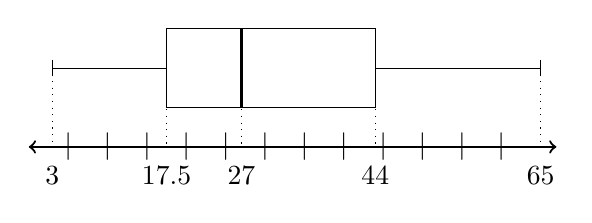
\begin{tikzpicture}[xscale=0.1]
      \def\median{27}
      \def\firstquartile{17.5}
      \def\thirdquartile{44}
      \def\minimum{3}
      \def\maximum{65}

      \draw (\firstquartile, -0.5 ) rectangle ( \thirdquartile,0.5);
      \draw[thick] ( \median,-0.5) -- ( \median,0.5);
      \draw (    \firstquartile, 0) -- (\minimum,0   );
      \draw ( \minimum, -0.1) -- (       \minimum, 0.1);
      \draw (  \thirdquartile, 0) -- (   \maximum, 0);
      \draw ( \maximum, -0.1) -- (      \maximum, 0.1 );

      \draw[thick,<->] (0,-1) -- (67,-1);

      \foreach \x in {\minimum, \firstquartile, \median, \thirdquartile, \maximum} {
        \draw (\x,-1.6) -- (\x, -1.6) node[anchor=south] {$\x$};
      }

      \foreach \x in {5,10,...,60} {
        \draw (\x,-1.3) -- (\x, -1.3) node[anchor=south] {$|$};
      }
      \draw[dotted] ( \maximum, 0.09) -- ( \maximum, -1);
      \draw[dotted] ( \thirdquartile, 0.49) -- ( \thirdquartile, -1);
      \draw[dotted] (\median, 0.49)  -- ( \median, -1);
      \draw[dotted] (\firstquartile, 0.49) -- ( \firstquartile, -1);
      \draw[dotted] ( \minimum, 0.09) -- ( \minimum, -1);
    \end{tikzpicture}
\item %Zithulele works as a telesales person. He keeps a record of the
%   number of sales he makes each month. The data below show how much he
%   sells each month.
%   \begin{equation*}
%     \{49;\ 12;\ 22;\ 35;\ 2;\ 45;\ 60;\ 48;\ 19;\ 1;\ 43;\ 12\}
%   \end{equation*}
%   Give the five number summary and box-and-whisker plot of Zithulele's
%   sales.
    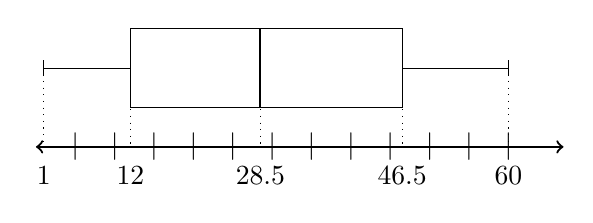
\begin{tikzpicture}[xscale=0.1]
      \def\median{28.5}
      \def\firstquartile{12}
      \def\thirdquartile{46.5}
      \def\minimum{1}
      \def\maximum{60}

      \draw (\firstquartile, -0.5 ) rectangle ( \thirdquartile,0.5);
      \draw[thick] ( \median,-0.5) -- ( \median,0.5);
      \draw (    \firstquartile, 0) -- (\minimum,0   );
      \draw ( \minimum, -0.1) -- (       \minimum, 0.1);
      \draw (  \thirdquartile, 0) -- (   \maximum, 0);
      \draw ( \maximum, -0.1) -- (      \maximum, 0.1 );

      \draw[thick,<->] (0,-1) -- (67,-1);

      \foreach \x in {\minimum, \firstquartile, \median, \thirdquartile, \maximum} {
        \draw (\x,-1.6) -- (\x, -1.6) node[anchor=south] {$\x$};
      }

      \foreach \x in {5,10,...,60} {
        \draw (\x,-1.3) -- (\x, -1.3) node[anchor=south] {$|$};
      }
      \draw[dotted] ( \maximum, 0.09) -- ( \maximum, -1);
      \draw[dotted] ( \thirdquartile, 0.49) -- ( \thirdquartile, -1);
      \draw[dotted] (\median, 0.49)  -- ( \median, -1);
      \draw[dotted] (\firstquartile, 0.49) -- ( \firstquartile, -1);
      \draw[dotted] ( \minimum, 0.09) -- ( \minimum, -1);
    \end{tikzpicture}
\item %Hannah has worked as a florist for nine months. She sold the
%   following number of wedding bouquets:
%   \begin{equation*}
%     \{16;\ 14;\ 8;\ 12;\ 6;\ 5;\ 3;\ 5;\ 7\}
%   \end{equation*}
%   Give the five number summary of Hannah's sales.
\item %Use the diagram below to determine the five number summary:
 \begin{enumerate}[noitemsep, label=\textbf{(\alph*)} ]
\item %


\item %

   
\end{enumerate}

\end{enumerate}
% }
% \end{exercises}

\subsection{End of chapter exercises} %p.307-309
% \begin{eocexercises}{}
  \begin{enumerate}[itemsep=6pt, label=\textbf{\arabic*}.]

  \item %
%   In a park, the tallest $7$ trees in a park have heights in metres of
%     $41$; $60$; $47$; $42$; $44$; $42$; and $47$. Find the median of
%     their heights.

  \item %The students in Ndeme's class have the following ages: $5$;
%     $6$; $7$; $5$; $4$; $6$; $6$; $6$; $7$; $4$. Find the mode of
%     their ages.

  \item %An engineering company has designed two different types of
%     engines for motorbikes. The two different motorbikes are tested
%     for the time (in seconds) it takes for them to accelerate from $0$
%     km/h to $60$ km/h.

    
\begin{enumerate}[noitemsep, label=\textbf{(\alph*)} ]
    \item %What measure of central tendency should be used for this
%       information?
    \item %Calculate the measure of central tendency that you chose in
%       the previous question, for each motorbike.
    \item %Which motorbike would you choose based on this information?
%       Take note of the accuracy of the numbers from each set of tests.
    \end{enumerate}

  \item %In a traffic survey, a random sample of $50$ motorists were
%     asked the distance they drove to work daily. This information is
%     shown in the table below.\\

     \begin{enumerate}[noitemsep, label=\textbf{(\alph*)} ]
    \item %Find the approximate mean of the data.
    \item %What percentage of samples had a speed of
      \begin{enumerate}[noitemsep, label=\textbf{\roman*}. ]
      \item %less than $16$ km?
      \item %more than $30$ km?
      \item %between $16$ km and $30$ km daily?
      \end{enumerate}
\item %Draw a histogram to represent the data
\scalebox{1} % Change this value to rescale the drawing.
{
\begin{pspicture}(0,-3.62375)(11.17442,3.58375)
\definecolor{color6331b}{rgb}{0.7725490196078432,0.7725490196078432,0.7725490196078432}
\psframe[linewidth=0.02,dimen=outer,fillstyle=solid,fillcolor=color6331b](2.208587,-0.41625)(1.1885868,-2.4128125)
\rput(1.1744202,-2.41625){\psaxes[linewidth=0.028222222,arrowsize=0.05291667cm 2.0,arrowlength=1.4,arrowinset=0.4,tickstyle=bottom,ticksize=0.10583333cm,dx=1.0cm,dy=0.5cm,Dx=5]{<->}(0,0)(-1,-1)(10,6)}
\psframe[linewidth=0.02,dimen=outer,fillstyle=solid,fillcolor=color6331b](3.188587,0.10375)(2.168587,-2.4128125)
\psframe[linewidth=0.02,dimen=outer,fillstyle=solid,fillcolor=color6331b](4.2085867,2.10375)(3.168587,-2.4128125)
\psframe[linewidth=0.02,dimen=outer,fillstyle=solid,fillcolor=color6331b](5.2085867,2.60375)(4.1685867,-2.4128125)
\psframe[linewidth=0.02,dimen=outer,fillstyle=solid,fillcolor=color6331b](6.1885867,1.12375)(5.1685867,-2.4128125)
\psframe[linewidth=0.02,dimen=outer,fillstyle=solid,fillcolor=color6331b](7.1885867,1.58375)(6.1685867,-2.4128125)
% \usefont{T1}{ptm}{m}{n}
\rput(6.062962,-3.42625){Distance (km)}
% \usefont{T1}{ptm}{m}{n}
\rput{89.854546}(1.2403736,0.9631185){\rput(0.11709099,1.0822288){Count}}
\psframe[linewidth=0.02,dimen=outer,fillstyle=solid,fillcolor=color6331b](8.188587,-0.89625)(7.1685867,-2.4128125)
\psframe[linewidth=0.02,dimen=outer,fillstyle=solid,fillcolor=color6331b](9.188587,-1.39625)(8.168587,-2.4128125)
\psframe[linewidth=0.02,dimen=outer,fillstyle=solid,fillcolor=color6331b](10.188587,-1.39625)(9.168587,-2.4128125)
\end{pspicture} 
}
    \end{enumerate}

  \item %A company wanted to evaluate the training programme in its
%     factory. They gave the same task to trained and untrained
%     employees and timed each one in seconds.

    \begin{enumerate}[noitemsep, label=\textbf{(\alph*)} ]
    \item %Find the medians and quartiles for both sets of data
    \item %Find the interquartile range for both sets of data
    \item %Comment on the results
\item %Draw two box-and-whisker diagrams to illustrate the five number summary
Trained employees:\\
    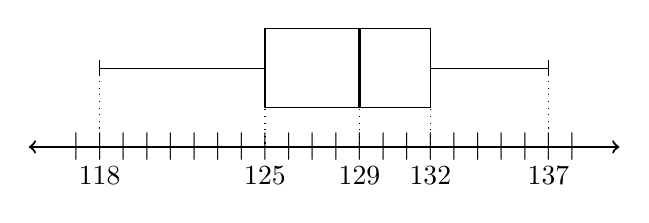
\begin{tikzpicture}[xscale=0.3]
      \def\median{129}
      \def\firstquartile{125}
      \def\thirdquartile{132}
      \def\minimum{118}
      \def\maximum{137}

      \draw (\firstquartile, -0.5 ) rectangle ( \thirdquartile,0.5);
      \draw[thick] ( \median,-0.5) -- ( \median,0.5);
      \draw (    \firstquartile, 0) -- (\minimum,0   );
      \draw ( \minimum, -0.1) -- (       \minimum, 0.1);
      \draw (  \thirdquartile, 0) -- (   \maximum, 0);
      \draw ( \maximum, -0.1) -- (      \maximum, 0.1 );

      \draw[thick,<->] (115,-1) -- (140,-1);

      \foreach \x in {\minimum, \firstquartile, \median, \thirdquartile, \maximum} {
        \draw (\x,-1.6) -- (\x, -1.6) node[anchor=south] {$\x$};
      }

      \foreach \x in {117,118,...,138} {
        \draw (\x,-1.3) -- (\x, -1.3) node[anchor=south] {$|$};
      }
      \draw[dotted] ( \maximum, 0.09) -- ( \maximum, -1);
      \draw[dotted] ( \thirdquartile, 0.49) -- ( \thirdquartile, -1);
      \draw[dotted] (\median, 0.49)  -- ( \median, -1);
      \draw[dotted] (\firstquartile, 0.49) -- ( \firstquartile, -1);
      \draw[dotted] ( \minimum, 0.09) -- ( \minimum, -1);
    \end{tikzpicture}
  
\\
Untrained employees:\\
    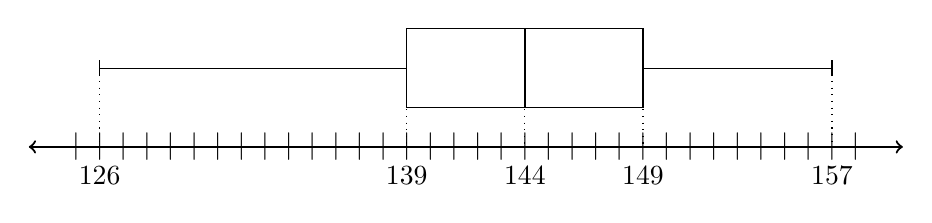
\begin{tikzpicture}[xscale=0.3]
      \def\median{144}
      \def\firstquartile{139}
      \def\thirdquartile{149}
      \def\minimum{126}
      \def\maximum{157}

      \draw (\firstquartile, -0.5 ) rectangle ( \thirdquartile,0.5);
      \draw[thick] ( \median,-0.5) -- ( \median,0.5);
      \draw (    \firstquartile, 0) -- (\minimum,0   );
      \draw ( \minimum, -0.1) -- (       \minimum, 0.1);
      \draw (  \thirdquartile, 0) -- (   \maximum, 0);
      \draw ( \maximum, -0.1) -- (      \maximum, 0.1 );

      \draw[thick,<->] (123,-1) -- (160,-1);

      \foreach \x in {\minimum, \firstquartile, \median, \thirdquartile, \maximum} {
        \draw (\x,-1.6) -- (\x, -1.6) node[anchor=south] {$\x$};
      }

      \foreach \x in {125,126,...,158} {
        \draw (\x,-1.3) -- (\x, -1.3) node[anchor=south] {$|$};
      }
      \draw[dotted] ( \maximum, 0.09) -- ( \maximum, -1);
      \draw[dotted] ( \thirdquartile, 0.49) -- ( \thirdquartile, -1);
      \draw[dotted] (\median, 0.49)  -- ( \median, -1);
      \draw[dotted] (\firstquartile, 0.49) -- ( \firstquartile, -1);
      \draw[dotted] ( \minimum, 0.09) -- ( \minimum, -1);
    \end{tikzpicture}
    \end{enumerate}

  \item %A small firm employs nine people. The annual salaries of the employers are:

    \begin{enumerate}[noitemsep, label=\textbf{(\alph*)} ]
    \item %Find the mean of these salaries
    \item %Find the mode
    \item %Find the median
    \item %Of these three figures, which would you use for
%       negotiating salary increases if you were a trade union
%       official? Why?
    \end{enumerate}

  \end{enumerate}
% \end{eocexercises}


\section {Probability}
\subsection{Exercise 10-1} %p. 316
% \begin{exercises}{}
% {
  \begin{enumerate}[itemsep=5pt, label=\textbf{\arabic*}. ]
  \item %
% A bag contains $6$ red, $3$ blue, $2$ green and $1$ white
%     balls. A ball is picked at random. Determine the probablity that it
%     is:
    \begin{enumerate}[noitemsep, label=\textbf{(\alph*)} ]
    \item %red
    \item %blue or white
    \item %not green
    \item %not green or red
    \end{enumerate}
  \item %
% A playing card is selected randomly from a pack of $52$
%     cards. Determine the probability that it is:
    \begin{enumerate}[noitemsep, label=\textbf{(\alph*)} ]
% \setcounter{enumi}{4}
    \item %the $2$ of hearts
    \item %a red card
    \item %a picture card
    \item %an ace
    \item %a number less than $4$?
    \end{enumerate}
\item %Even numbers in the range $2$--$100$ are written on cards. 
%What is
%     the probability of selecting a multiple of $5$, if a card is drawn
%     at random?

\end{enumerate}
% }
% \end{exercises}
\subsection{Exercise 10-2} %p. 323
% \begin{exercises}{}
% {
    \begin{enumerate}[itemsep=5pt, label=\textbf{\arabic*}. ]
   \item %Let $S$ denote the set of whole numbers from $1$ to $16$, $X$
%     denote the set of even numbers from $1$ to $16$ and $Y$ denote the
%     set of prime numbers from $1$ to $16$
 %Draw a Venn diagram accurately depicting $S$, $X$ and $Y$.
%     \item %Find $n\left(S\right)$, $n\left(X\right)$, $n\left(Y\right)$,
%       $n\left(X\cup Y\right)$, $n\left(X\cap Y\right)$.
%     \end{enumerate}
\item
%   There are $79$ Grade $10$ learners at school. All of these
%     take some combination of Maths, Geography and History. The number who take
%     Geography is $41$, those who take History is $36$, and $30$ take
%     Maths. The number who take Maths and History is $16$; the number
%     who take Geography and History is $6$, and there are $8$ who take
%     Maths only and $16$ who take only History.
    \begin{enumerate}[noitemsep, label=\textbf{(\alph*)} ]

    \item %Draw a Venn diagram to illustrate all this information.
    \item %How many learners take Maths and Geography but not History?
    \item %How many learners take Geography only?
    \item %How many learners take all three subjects?
    \end{enumerate}
 \item %Pieces of paper labelled with the numbers $1$ to $12$ are
%     placed in a box and the box is shaken. One piece of paper is taken
%     out and then replaced.
    \begin{enumerate}[noitemsep, label=\textbf{(\alph*)} ]

    \item %What is the sample space, $S$?
    \item %Write down the set $A$, representing the event of taking a
%       piece of paper labelled with a factor of $12$.
    \item %Write down the set $B$, representing the event of taking a
%       piece of paper labelled with a prime number.
    \item %Represent $A$, $B$ and $S$ by means of a Venn diagram.
    \item %Find
      \begin{enumerate}[noitemsep, label=\textbf{\roman*.} ]
      \item %$n\left(S\right)$
      \item %$n\left(A\right)$
      \item %$n\left(B\right)$
%       \item %$n\left(A\cap B\right)$
%       \item %$n\left(A\cup B\right)$
      \end{enumerate}
%     \item %Is $n\left(A\cup B\right)=n\left(A\right)+n\left(B\right)-n\left(A\cap B\right)$?
    \end{enumerate}
  \end{enumerate}

% }
% \end{exercises}
\subsection{Exercise 10-3} %p. 331-332
% \begin{exercises}{}
% {
\begin{enumerate}[itemsep=6pt, label=\textbf{\arabic*}. ] 
  \item %A box contains coloured blocks. The number of each colour is
%     given in the following table.

   \item %A block is selected randomly. What is the probability that the block will be:
  \begin{enumerate}[noitemsep, label=\textbf{(\alph*)} ]
    \item %purple
    \item %purple or white
    \item %pink and orange
    \item %not orange?
    \end{enumerate}

  \item %A small school has a class with children of various ages. The
%     table gives the number of pupils of each age in the class.

   
%     If a pupil is selected at random what is the probability that the
%     pupil will be:
  \begin{enumerate}[noitemsep, label=\textbf{(\alph*)} ]

    \item %a female
    \item %a $4$ year old male
    \item %aged $3$ or $4$
    \item %aged $3$ and $4$
    \item %not $5$
    \item %either $3$ or female?
    \end{enumerate}
\item
% Fiona has $85$ labeled discs, which are numbered from $1$ to
%     $85$. If a disc is selected at random what is the probability that
%     the disc number:
  \begin{enumerate}[noitemsep, label=\textbf{(\alph*)} ]
% \setcounter{enumi}{10}
    \item %ends with $5$
    \item %can be multiplied by $3$
    \item %can be multiplied by $6$
    \item %is number $65$
    \item %is not a multiple of $5$
    \item %is a multiple of $4$ or $3$
    \item %is a multiple of $2$ and $6$
    \item %is number $1$?
    \end{enumerate}

 \end{enumerate}
% }
% \end{exercises}
\subsection{End of chapter exercises} %p.333-335

% \begin{eocexercises}{}
  \begin{enumerate}[itemsep=5pt, label=\textbf{\arabic*}. ]
  \item %A group of $45$ children were asked if they eat Frosties and/or
%     Strawberry Pops. $31$ eat both and $6$ eat only Frosties. What is the
%     probability that a child chosen at random will eat only Strawberry
%     Pops?
  \item %In a group of $42$ pupils, all but $3$ had a packet of chips
%     or a Fanta or both. If $23$ had a packet of chips and $7$ of these
%     also had a Fanta, what is the probability that one pupil chosen at
%     random has:
    \begin{enumerate}[noitemsep, label=\textbf{(\alph*)} ]
    \item %both chips and Fanta
    \item %only Fanta?
    \end{enumerate}
  \item %Use a Venn diagram to work out the following probabilities
%     from a die be rolled:
    \begin{enumerate}[noitemsep, label=\textbf{(\alph*)} ]
    \item %a multiple of $5$ and an odd number
    \item %a number that is neither a multiple of $5$ nor an odd
%       number
    \item %a number which is not a multiple of $5$, but is odd
    \end{enumerate}
  \item %A packet has yellow and pink sweets. The probability of taking
%     out a pink sweet is $\frac{7}{12}$.
    \begin{enumerate}[noitemsep, label=\textbf{(\alph*)} ]
    \item %What is the probability of taking out a yellow sweet
    \item %If $44$ if the sweets are yellow, how many sweets are pink?
    \end{enumerate}
  \item %In a car park with $300$ cars, there are $190$ Opels. What is the
%     probability that the first car to leave the car park is:
    \begin{enumerate}[noitemsep, label=\textbf{(\alph*)} ]
    \item %an Opel
    \item %not an Opel
    \end{enumerate}
  \item %Tamara has $18$ loose socks in a drawer. Eight of these are
%     orange and two are pink. Calculate the probability that the first
%     sock taken out at random is:
    \begin{enumerate}[noitemsep, label=\textbf{(\alph*)} ]
    \item %orange
    \item %not orange
    \item %pink
    \item %not pink
    \item %orange or pink
    \item %neither orange nor pink
    \end{enumerate}
  \item %A plate contains $9$ shortbread cookies, $4$ ginger biscuits,
%     $11$ chocolate chip cookies and $18$ Jambos. If a biscuit is
%     selected at random, what is the probability that:
    \begin{enumerate}[noitemsep, label=\textbf{(\alph*)} ]
    \item %it is either a ginger biscuit of a Jambo
    \item %it is not a shortbread cookie
    \end{enumerate}
  \item %$280$ tickets were sold at a raffle. Ingrid bought $15$
%     tickets. What is the probability that Ingrid:
    \begin{enumerate}[noitemsep, label=\textbf{(\alph*)} ]
    \item %wins the prize
    \item %does not win the prize
    \end{enumerate}
  \item %The children in a nursery school were classified by hair and
%     eye colour. $44$ had red hair and not brown eyes, $14$ had brown eyes
%     and red hair, $5$ had brown eyes but not red hair and $40$ did not
%     have brown eyes or red hair.
    \begin{enumerate}[noitemsep, label=\textbf{(\alph*)} ]
    \item %how many children were in the schoo?
    \item %What is the probility that a child chosen at random has:
      \begin{enumerate}
      \item %brown eyes
      \item %red hair
      \end{enumerate} 
    \item %A child with brown eyes is chosen randomly. What is the
%       probability that this child will have red hair?
    \end{enumerate}
  \item %A jar has purple, blue and black sweets in it. The probability
%     that a sweet chosen at random will be purple is $\frac{1}{7}$
%     and the probability that it will be black is $\frac{3}{5}$.
    \begin{enumerate}[noitemsep, label=\textbf{(\alph*)} ]
\item %If I choose a sweet at random what
%       is the probability that it will be:
      \begin{enumerate}
      \item %purple or blue
      \item %black
      \item %purple
      \end{enumerate}
    \item %If there are $70$ sweets in the jar how many purple ones are       there?
    \item %$\frac{1}{4}$ of the purple sweets in b) have streaks on
%       them and the rest do not. How many purple sweets have streaks?
    \end{enumerate}
\item %For each of the following, draw a Venn diagram to represent
%     the situation and find an example to illustrate the situation.
    \begin{enumerate}[noitemsep, label=\textbf{(\alph*)} ]
    \item %a sample space in which there are two events that are not
%       mutually exclusive
    \item %a sample space in which there are two events that are
%       complementary
    \end{enumerate}
\item %Use a Venn diagram to prove that the probability of either
%     event $A$ or $B$ occuring is given by: ($A$ and $B$ are not
%     exclusive)
%     \[P(A \cup B) = P(A) + P(B) - P(A \cap B)\]
\item %All the clubs are taken out of a pack of cards. The remaining
%     cards are then shuffled and one card chosen. After being chosen,
%     the card is replaced before the next card is chosen.
    \begin{enumerate}[noitemsep, label=\textbf{(\alph*)} ]
    \item %What is the sample space?
    \item %Find a set to represent the event, $P$, of drawing a picture
%       card.
    \item %Find a set for the event, $N$, of drawing a numbered card.
    \item %Represent the above events in a Venn diagram.
    \item %What description of the sets $P$ and $N$ is suitable?
%       (Hint: Find any elements of $P$ in $N$ and of $N$ in $P$.)
    \end{enumerate}
\item %Thuli has a bag containing five orange, three purple and seven
%     pink blocks. The bag is shaken and a block is withdrawn. The
%     colour of the block is noted and the block is replaced.
    \begin{enumerate}[noitemsep, label=\textbf{(\alph*)} ]
    \item %What is the sample space for this experiment?
    \item %What is the set describing the event of drawing a pink
%       block, $P$?
    \item %Write down a set, $O$ or $B$, to represent the event of
%       drawing either a orange or a purple block.
    \item %Draw a Venn diagram to show the above information.
    \end{enumerate}
  \end{enumerate}

% \end{eocexercises}




\section {Euclidean geometry}
\subsection{Exercise 11-1} %p. 342-344
% \begin{exercises}{}
% {
       
\begin{enumerate}[label=\textbf{\arabic*}.]
\item %Use adjacent, corresponding, co-interior and alternate angles to fill in all the angles labeled with letters in the diagram:\\

\item %Find all the unknown angles in the figure: \\

 
\item %Find the value of $x$ in the figure: \\


\item %Determine whether the pairs of lines in the following figures are parallel:
\begin{enumerate}[itemsep=10pt, label=\textbf{(\alph*)} ] 
            \item %

\item %

    \item %

    \end{enumerate}
\item %If $AB$ is parallel to $CD$ and $AB$ is parallel to $EF$, explain why $CD$ must be parallel to $EF$.\vspace{8pt}\\
\end{enumerate}
% }
% \end{exercises}
\subsection{Exercise 11-2} %p. 351-352
% \begin{exercises}{}{
 \begin{enumerate}[itemsep=5pt, label=\textbf{\arabic*}. ]
  \item %Calculate the unknown variables in each of the following figures.
\begin{enumerate}[noitemsep, label=\textbf{(\alph*)} ]
\item
\item
\item
\item
\item
\item
\item
\item
\end{enumerate}
\item %State whether the following pairs of triangles are congruent or not. Give reasons for your answers. If there is not enough information to make a descision, explain why.
\begin{enumerate}[noitemsep, label=\textbf{(\alph*)} ]

\item
\item
\item
\item
\item
\end{enumerate}

\end{enumerate}
% }
% \end{exercises}
\subsection{Exercise 11-3}
  \begin{enumerate}[itemsep=5pt, label=\textbf{\arabic*}. ]
 \item %Prove that the diagonals of the parallelogram $MNRS$ bisect one another at $P$. \\
\end{enumerate}

\subsection{Exercise 11-4} %p. 357
% \begin{exercises}{}
% {
  \begin{enumerate}[itemsep=5pt, label=\textbf{\arabic*}. ]
   \item
% 
% $ABCD$ is a quadrilateral. Diagonals $AC$ and $BD$ intersect at $T$. $AC = BD$, $AT=TC$, $DT=TB$. Prove that:
\begin{enumerate}[noitemsep, label=\textbf{(\alph*)} ]
\item %$ABCD$ is a parallelogram.
\item %$ABCD$ is a rectangle.
\end{enumerate}

\end{enumerate}
% }
% \end{exercises}

\subsection{Exercise 11-5} %p. 359
% \begin{exercises}{}
% {
\begin{enumerate}[itemsep=10pt, label=\textbf{\arabic*}.]
 \item %Use the sketch of kite $ABCD$ to prove the diagonals are perpendicular to one another.\\

\item
% Explain why quadrilateral $WXYZ$ is a kite. Write down all the properties of quadrilateral $WXYZ$.\\

\end{enumerate}
% }
% \end{exercises}
\subsection{Exercise 11-6} %p. 366
% \begin{exercises}{}{
\begin{enumerate}[itemsep=6pt,label=\textbf{\arabic*}.]
\item % Find $x$ and $y$ in each of the following:\\
\begin{enumerate}[noitemsep, label=\textbf{(\alph*)} ]

\item
\item
\item
\item
\item
\end{enumerate}

% \setcounter{enumi}{5}
\item %Show that $M$ is the mid-point of $AB$ and that $MN=RC$.\\



\item %$ABCD$ is a rhombus with $AM = MO$ and $AN = NO$. Prove $ANOM$ is a rhombus.\\

\end{enumerate}
}
\end{exercises}

\subsection{End of chapter exercises} %p.374-379
% \begin{eocexercises}{}

\begin{enumerate}[itemsep=20pt, label=\textbf{\arabic*}.]
%First question
\item %Identify the types of angles shown below:\\
\begin{enumerate}[noitemsep, label=\textbf{(\alph*)} ]
\item
\item
\item
\item
\item
\item
\item
\item
\end{enumerate}

\item %Assess whether the following statements are true or false. If the
% statement is false, explain why:
   \begin{enumerate}[noitemsep, label=\textbf{(\alph*)} ]
% \setcounter{enumi}{8}
\item % A trapezium is a quadrilateral with two pairs of opposite sides that are parallel.
\item % Both diagonals of a parallelogram bisect each other.
\item % A rectangle is a parallelogram that has one corner angles equal to $90^{\circ}$.
\item % Two adjacent sides of a rhombus have different lengths.
\item % The diagonals of a kite intersect at right angles.
\item %All squares are parallelograms.
\item %A rhombus is a kite with a pair of equal, opposite sides.
\item %The diagonals of a parallelogram are axes of symmetry.
\item %The diagonals of a rhombus are equal in length.
\item %Both diagonals of a kite bisect the interior angles.
\end{enumerate}
%Third question
\item %Calculate the size of the third angle ($x$) in each of the diagrams below:\\
\begin{enumerate}[noitemsep, label=\textbf{(\alph*)} ]
\item
\item
\item
\item
\item
\item
\end{enumerate}

%Question 4
\item %Find all the pairs of parallel lines in the following figures, giving reasons in each case.
\begin{enumerate}[noitemsep, label=\textbf{(\alph*)} ]
\item
\item
\item
\end{enumerate}
% Question 5

\item %Find angles $a$, $b$, $c$ and $d$ in each case, giving reasons:\\
\begin{enumerate}[noitemsep, label=\textbf{(\alph*)} ]
\item
\item
\item
\end{enumerate}

%Question 6
\item %Say which of the following pairs of triangles are congruent with reasons. 

  \begin{enumerate}[itemsep=6pt, label=\textbf{(\alph*)} ]
% \setcounter{enumi}{30}
\item %

\item %

\item %
\
\item %

\end{enumerate}

%Question 7 
\item %Using Pythagoras' theorem for right-angled triangles, calculate the length $x$:
   \begin{enumerate}[itemsep=8pt, label=\textbf{(\alph*)} ]
% \setcounter{enumi}{34}
\item %

\item %

\item %

\item %

\end{enumerate}
%Question 8
\item %Consider the diagram below. Is $\triangle ABC ||| \triangle DEF$? Give reasons for your answer. \\



%Question 9
\item %Explain why $\triangle PQR$ is similar to $\triangle TRS$ and calculate the values of $x$ and $y$.\\


\item %Calculate $a$ and $b$:\\


\item

% $ABCD$ is a parallelogram with diagonal $AC$.\\
% Given that $AF=HC$, show that:
   \begin{enumerate}[noitemsep, label=\textbf{(\alph*)} ]
 \item %$\triangle AFD \equiv \triangle CHB$
\item %$DF\parallel HB$
\item %$DFBH$ is a parallelogram
\end{enumerate}



\item % $\triangle PQR$ and $\triangle PSR$ are equilateral triangles. Prove that $PQRS$ is a rhombus:\\

\item %Given parallelogram $ABCD$ with $AE$ and $FC$, $AE$ bisects $\hat{A}$ and $FC$ bisects $\hat{C}$.
   \begin{enumerate}[noitemsep, label=\textbf{(\alph*)} ]
 \item %Write all interior angles in terms of $y$.
\item %Prove that $AFCE$ is a parallelogram.
\end{enumerate}

\item %Given that $WZ=ZY=YX$ and $WZ \parallel ZY$, prove that:
   \begin{enumerate}[noitemsep, label=\textbf{(\alph*)} ]
\item %$XZ$ bisects $\hat{X}$
\item %$WY=YZ$
% \begin{figure}[H]

\end{enumerate}

\item %$LMAO$ is a quadrilateral with $LM=LO$ and diagonals that intersect at $S$ such that $MS=SO$. Prove that:
   \begin{enumerate}[noitemsep, label=\textbf{(\alph*)} ]
% \setcounter{enumi}{49}
 \item %$M\hat{L}S = S\hat{L}O$
\item %$\triangle LOA \equiv \triangle LMA$
\item %$MO \perp LA$
% \begin{figure}[H]

% \end{figure}
\end{enumerate}


%Challenge
\item %\textbf{Challenge problem:} Using the figure below, show that the sum of the three angles in a triangle is 180$^{\circ }$. Line $DE$ is parallel to $BC$.\\

\end{enumerate}

% \end{eocexercises}
\section {Measurements}
\subsection{Exercise 12-1} %p. 384-385
% \begin{exercises}{}
% {

% Find the areas of each of the polygons below:
\begin{enumerate}[noitemsep, label=\textbf{\arabic*}. ] 
 \item
\item
\item
\item 
\item
\item
\item
\item 
\end{enumerate}
% }
% \end{exercises}
\subsection{Exercise 12-2} %p. 393-394
% \begin{exercises}{ }{
\begin{enumerate}[noitemsep, label=\textbf{\arabic*}. ] 
\item %Calculate the surface area of the following prisms:
 \begin{enumerate}[noitemsep, label=\textbf{(\alph*)} ]
  \item 
\item 
\item
 \end{enumerate}


\item %If a litre of paint covers an area of $2$ m$^{2}$, how much paint does a painter need to cover:
 \begin{enumerate}[noitemsep, label=\textbf{(\alph*)} ]
% \setcounter{enumi}{3}
\item %a rectangular swimming pool with dimensions $4$ m $\times~3$ m $\times~2,5$ m (the inside walls and floor only).
\item %the inside walls and floor of a circular reservoir with diameter $4$ m and height $2,5$ m.
\end{enumerate}


 \end{enumerate}       
% }
% \end{exercises} 
\subsection{Exercise 12-3} %p. 398
% \begin{exercises}{}{
% Calculate the volumes of the following prisms (correct to one decimal place):
\begin{enumerate}[itemsep=6pt, label=\textbf{\arabic*}. ] 
\item
\item
\item
\end{enumerate}
% }
% \end{exercises}
\subsection{Exercise 12-4} %p. 417-418
% \begin{exercises}{}
%  {
\begin{enumerate}[itemsep=6pt, label=\textbf{\arabic*}. ] 
\item %Find the total surface area of the following objects (correct to $1$ decimal place if necessary):
\begin{enumerate}[noitemsep, label=\textbf{\alph*}. ]
 \item
\item
\item 
\item
\end{enumerate}
\item % Find the volume of the following objects (round off to $1$ decimal place if needed):
\begin{enumerate}[noitemsep, label=\textbf{\alph*}. ]
 \item
\item
\item 
\item
\end{enumerate}
\item %This solid  is made up of a cube and a square pyramid. Find it's volume and surface area (correct to $1$ decimal place):

\end{enumerate}
% }
% \end{exercises}
\subsection{Exercise 12-5} %p. 425
% \begin{exercises}{}
%  {
\begin{enumerate}[noitemsep, label=\textbf{\arabic*}. ] 
 \item %If the height of a prism is doubled, how much will its volume increase?
\item %Describe the change in the volume of a rectangular prism if:
\begin{enumerate}[noitemsep, label=\textbf{(\alph*)} ] 
\item %length and breadth increase by a constant factor of $3$
\item %length, breadth and height are multiplied by a constant factor of $2$
\end{enumerate}
\item %Given a prism with a volume of $493$ cm$^{3}$ and a surface area of $6007$ cm$^{2}$, find the new surface area and volume for a prism if all dimensions are increased by a constant factor of $4$. 
\end{enumerate}
% 
% }
% \end{exercises}

\subsection{End of chapter exercises} %p.426-427
% \begin{eocexercises}{}

\begin{enumerate}[itemsep=6pt, label=\textbf{\arabic*}. ] 
\item %Consider the solids below and answer the questions that follow (correct to one decimal place, if necessary):

    \begin{enumerate}[noitemsep, label=\textbf{(\alph*)} ]
  \item %Calculate the surface area of each solid.
\item %Calculate volume of each solid.
\item %If each dimension of the solid is increased by a factor of $3$, calculate the new surface area of each solid.
\item %If each dimension of the solid is increased by a factor of $3$, calculate the new volume of each solid.
 \end{enumerate}
\item %Consider the solids below:

    \begin{enumerate}[noitemsep, label=\textbf{(\alph*)} ]
% \setcounter{enumi}{4}
 \item %Calculate the surface area of each solid.
\item %Calculate the volume of each solid.

\end{enumerate}

% \setcounter{enumi}{6}
\item %Calculate the volume and surface area of the solid below (correct to $1$ decimal place):
\end{enumerate}

% }
% \end{eocexercises}